% This is samplepaper.tex, a sample chapter demonstrating the
% LLNCS macro package for Springer Computer Science proceedings;
% Version 2.20 of 2017/10/04
%
\documentclass[12pt,a4paper,roman]{article}
%

\usepackage{geometry}
\geometry{a4paper, margin=3cm}

\usepackage{amsmath}
\usepackage{amssymb}
\usepackage{booktabs} % For pretty tables
\usepackage{caption} % For caption spacing
\usepackage{subcaption} % For sub-figures
\usepackage{graphicx}
\usepackage{mathtools}
\graphicspath{ {./figures/} }
\usepackage{pgfplots}
\usepackage[all]{nowidow}
\usepackage[utf8]{inputenc}
\usepackage{xcolor}
\usepackage{multicol}
\usepackage{algpseudocode,algorithm,algorithmicx}
\usepackage{hyperref}
\usepackage{cleveref}
\usepackage[inline]{enumitem} % Horizontal lists
% Used for displaying a sample figure. If possible, figure files should
% be included in EPS format.
%
% If you use the hyperref package, please uncomment the following line
% to display URLs in blue roman font according to Springer's eBook style:
% \renewcommand\UrlFont{\color{blue}\rmfamily}
\newcommand{\defeq}{\vcentcolon=}
\newcommand{\eqdef}{=\vcentcolon}
\newcommand{\card}[1]{\left\vert{#1}\right\vert}
\newcommand*\Let[2]{\State #1 $\gets$ #2}
\definecolor{blue}{HTML}{1F77B4}
\definecolor{orange}{HTML}{FF7F0E}
\definecolor{green}{HTML}{2CA02C}



% colors
\definecolor{blau}{RGB}{0,84,159}
\definecolor{maigruen}{RGB}{189,205,0}
\definecolor{rot}{RGB}{204,7,30}
\definecolor{bordeaux}{RGB}{161,16,53}
\definecolor{violett}{RGB}{97,33,88}
\definecolor{lila}{RGB}{122,111,172}
\definecolor{magenta}{RGB}{255,0,255}
\definecolor{orange}{RGB}{255,140,0}

\definecolor{gelb}{RGB}{247,166,60}
\definecolor{gruen}{RGB}{85,170,67}
\definecolor{rot2}{RGB}{205,2,37}        %%%%
\definecolor{blau2}{RGB}{0,86,153}      %%%%

\newcommand{\bl}[1]{{\color{blau}{#1}}}
\newcommand{\vl}[1]{{\color{violett}{#1}}}
\newcommand{\gr}[1]{{\color{Green}{#1}}}
\newcommand{\rd}[1]{{\color{rot}{#1}}}
\newcommand{\bd}[1]{{\color{bordeaux}{#1}}}
\newcommand{\mg}[1]{{\color{magenta}{#1}}}
\newcommand{\ora}[1]{{\color{orange}{#1}}}

%  diagrammatic classes
\newcommand{\K}[1]{\mathcal{K}_#1}
\newcommand{\Ka}[1]{\mathcal{K}_#1^a}
\newcommand{\Kp}[1]{\mathcal{K}_#1^p}
\newcommand{\Kt}[1]{\mathcal{K}_#1^t}
\newcommand{\Kbar}[1]{\bar{\mathcal{K}}_#1}
\newcommand{\Kabar}[1]{\bar{\mathcal{K}}_#1^a}
\newcommand{\Kpbar}[1]{\bar{\mathcal{K}}_#1^p}
\newcommand{\Ktbar}[1]{\bar{\mathcal{K}}_#1^t}

\newcommand{\al}[6]{
	^{
		\ifcase #5 %0
		\alpha_#1 \alpha_#2 
		\or %1
		\alpha_#1^\prime \alpha_#2^\prime 
		\or %2
		#1 #2
		\or %3
		\bar{\alpha}_#1 \alpha_#2
		\or %4
		\alpha_#1 \bar{\alpha}_#2
		\or %5
		\bar{\alpha}_#1 \bar{\alpha}_#2
		\or %6
		\bar{\alpha}_#1^\prime \alpha_#2^\prime
		\or %7
		\alpha_#1^\prime \bar{\alpha}_#2^\prime
		\or %8
		\bar{\alpha}_#1^\prime \bar{\alpha}_#2^\prime
		\else
		0
		\fi
		|
		\ifcase #6 %0
		\alpha_#3 \alpha_#4
		\or %1
		\alpha_#3^\prime \alpha_#4^\prime
		\or %2
		#3 #4
		\or %3
		\bar{\alpha}_#3 \alpha_#4
		\or %4
		\alpha_#3 \bar{\alpha}_#4
		\or %5
		\bar{\alpha}_#3 \bar{\alpha}_#4
		\or %6
		\bar{\alpha}_#3^\prime \alpha_#4^\prime
		\or %7
		\alpha_#3^\prime \bar{\alpha}_#4^\prime
		\or %8
		\bar{\alpha}_#3^\prime \bar{\alpha}_#4^\prime
		\else
		0
		\fi
	}
}
%
% sigma: 
% 0 = sigma_ind
% 1 = sigma_ind^\prime
% 2 = ind (no sigma)
\newcommand{\si}[6]{
	_{
		\ifcase #5
		\sigma_#1 \sigma_#2 
		\or
		\sigma_#1^\prime \sigma_#2^\prime 
		\or
		#1 #2
		\else
		0
		\fi
		|
		\ifcase #6
		\sigma_#3 \sigma_#4
		\or
		\sigma_#3^\prime \sigma_#4^\prime
		\or
		#3 #4
		\else
		0
		\fi
	}
}
%
% sigmas:
% 0 = sigma sigma
% 1 = sigma \bar{sigma}
% 2 = \bar{sigma} sigma
\newcommand{\sig}[2]{
	_{
		\ifcase #1
		\sigma \sigma
		\or
		\sigma \bar{\sigma}
		\or
		\bar{\sigma} \sigma
		\else
		0
		\fi
		|
		\ifcase #2
		\sigma \sigma
		\or
		\sigma \bar{\sigma}
		\or
		\bar{\sigma} \sigma
		\else
		0
		\fi
	}
}
%
\newcommand{\sss}{_{\sigma \sigma}}
\newcommand{\ssb}{_{\sigma \bar{\sigma}}}
\newcommand{\sbs}{_{\bar{\sigma} \sigma}}
\newcommand{\ass}[1][]{_{a_{#1}, \sigma \sigma}}
\newcommand{\asb}[1][]{_{a_{#1}, \sigma \bar{\sigma}}}
\newcommand{\abs}[1][]{_{a_{#1}, \bar{\sigma} \sigma}}
\newcommand{\pss}[1][]{_{p_{#1}, \sigma \sigma}}
\newcommand{\psb}[1][]{_{p_{#1}, \sigma \bar{\sigma}}}
\newcommand{\pbs}[1][]{_{p_{#1}, \bar{\sigma} \sigma}}
\newcommand{\tss}[1][]{_{t_{#1}, \sigma \sigma}}
\newcommand{\tsb}[1][]{_{t_{#1}, \sigma \bar{\sigma}}}
\newcommand{\tbs}[1][]{_{t_{#1}, \bar{\sigma} \sigma}}

\newcommand{\q}[6]{
	\ifcase #5
	q_#1 q_#2 
	\or
	q_#1^\prime q_#2^\prime 
	\else
	0
	\fi
	|
	\ifcase #6
	q_#3 q_#4
	\or
	q_#3^\prime q_#4^\prime
	\else
	0
	\fi
	\,,\,
}
\newcommand{\om}[6]{
	\ifcase #5
	\omega_#1 \omega_#2 
	\or
	\omega_#1^\prime \omega_#2^\prime 
	\else
	0
	\fi
	|
	\ifcase #6
	\omega_#3 \omega_#4
	\or
	\omega_#3^\prime \omega_#4^\prime
	\else
	0
	\fi
}

\newcommand{\V}[9]{
	\def\Vertex{#1}
	\def\ala{#2}
	\def\alb{#3}
	\def\alc{#4}
	\def\ald{#5}
	\def\sga{#6}
	\def\sgb{#7}
	\def\sgc{#8}
	\def\sgd{#9}
	\Vcont
}

\newcommand{\vqw}[8]{
	\def\qa{#1}
	\def\qb{#2}
	\def\qc{#3}
	\def\qd{#4}
	\def\wa{#5}
	\def\wb{#6}
	\def\wc{#7}
	\def\wd{#8}
	\vqwcont
}

% independent Keldysh components in different diagrammatic classes

\definecolor{Aa}{RGB}{0, 0, 102}%{0,97,101}
\definecolor{Ba}{RGB}{51, 51, 153}
\definecolor{Ca}{RGB}{102,102,153}%{97,33,88}
\definecolor{Da}{RGB}{102, 0, 204}
\definecolor{Ea}{RGB}{153, 0, 255}
\definecolor{Fa}{RGB}{204, 0, 255}

\definecolor{Ap}{RGB}{153, 51, 51}%{87,171,39}
\definecolor{Bp}{RGB}{128, 0, 0}
\definecolor{Cp}{RGB}{255, 0, 0}%{204,7,30}
\definecolor{Dp}{RGB}{255, 102, 0}
\definecolor{Ep}{RGB}{255, 153, 51}
\definecolor{Fp}{RGB}{255, 204, 0}

\definecolor{At}{RGB}{0, 51, 0}%{189,205,0}
\definecolor{Bt}{RGB}{0, 102, 0}
\definecolor{Ct}{RGB}{51, 153, 51}%{246,168,0}
\definecolor{Dt}{RGB}{51, 153, 102}
\definecolor{Et}{RGB}{0, 204, 102}
\definecolor{Ft}{RGB}{0, 255, 0}

\newcommand{\Aa}[1]{{\color{Aa} $A_{#1}^a$}}
\newcommand{\Ap}[1]{{\color{Ap} $A_{#1}^p$}}
\newcommand{\At}[1]{{\color{At} $A_{#1}^t$}}
\newcommand{\Ba}[1]{{\color{Ba} $B_{#1}^a$}}
\newcommand{\Bp}[1]{{\color{Bp} $B_{#1}^p$}}
\newcommand{\Bt}[1]{{\color{Bt} $B_{#1}^t$}}
\newcommand{\Ca}[1]{{\color{Ca} $C_{#1}^a$}}
\newcommand{\Cp}[1]{{\color{Cp} $C_{#1}^p$}}
\newcommand{\Ct}[1]{{\color{Ct} $C_{#1}^t$}}
\newcommand{\Da}[1]{{\color{Da} $D_{#1}^a$}}
\newcommand{\Dp}[1]{{\color{Dp} $D_{#1}^p$}}
\newcommand{\Dt}[1]{{\color{Dt} $D_{#1}^t$}}
\newcommand{\Fa}[1]{{\color{Fa} $F_{#1}^a$}}
\newcommand{\Fp}[1]{{\color{Fp} $F_{#1}^p$}}
\newcommand{\Ft}[1]{{\color{Ft} $F_{#1}^t$}}

\newcommand{\bAa}[1]{{\color{Aa} $\bar{A}_{#1}^a$}}
\newcommand{\bAp}[1]{{\color{Ap} $\bar{A}_{#1}^p$}}
\newcommand{\bAt}[1]{{\color{At} $\bar{A}_{#1}^t$}}
\newcommand{\bBa}[1]{{\color{Ba} $\bar{B}_{#1}^a$}}
\newcommand{\bBp}[1]{{\color{Bp} $\bar{B}_{#1}^p$}}
\newcommand{\bBt}[1]{{\color{Bt} $\bar{B}_{#1}^t$}}
\newcommand{\bCa}[1]{{\color{Ca} $\bar{C}_{#1}^a$}}
\newcommand{\bCp}[1]{{\color{Cp} $\bar{C}_{#1}^p$}}
\newcommand{\bCt}[1]{{\color{Ct} $\bar{C}_{#1}^t$}}
\newcommand{\bDa}[1]{{\color{Da} $\bar{D}_{#1}^a$}}
\newcommand{\bDp}[1]{{\color{Dp} $\bar{D}_{#1}^p$}}
\newcommand{\bDt}[1]{{\color{Dt} $\bar{D}_{#1}^t$}}
\newcommand{\bEa}[1]{{\color{Ea} $\bar{E}_{#1}^a$}}
\newcommand{\bEp}[1]{{\color{Ep} $\bar{E}_{#1}^p$}}
\newcommand{\bEt}[1]{{\color{Et} $\bar{E}_{#1}^t$}}
\newcommand{\bFa}[1]{{\color{Fa} $\bar{F}_{#1}^a$}}
\newcommand{\bFp}[1]{{\color{Fp} $\bar{F}_{#1}^p$}}
\newcommand{\bFt}[1]{{\color{Ft} $\bar{F}_{#1}^t$}}

\newcommand{\dd}{\mathrm{d}}

\renewcommand{\topfraction}{0.85}
\renewcommand{\bottomfraction}{0.85}
\renewcommand{\textfraction}{0.15}
\renewcommand{\floatpagefraction}{0.8}
\renewcommand{\textfraction}{0.1}
\setlength{\floatsep}{3pt plus 1pt minus 1pt}
\setlength{\textfloatsep}{3pt plus 1pt minus 1pt}
\setlength{\intextsep}{3pt plus 1pt minus 1pt}
\setlength{\abovecaptionskip}{2pt plus 1pt minus 1pt}

\begin{document}
%
\title{Keldysh vertices and mfRG flow equations}
%
%\titlerunning{Abbreviated paper title}
% If the paper title is too long for the running head, you can set
% an abbreviated paper title here
%
\author{Santiago Aguirre \& Elias Walter}
%
%\authorrunning{F. Author et al.}
% First names are abbreviated in the running head.
% If there are more than two authors, 'et al.' is used.
%
%\institute{Ludwig-Maximilians University, Munich, Germany \\
%\email{\{sa.aguirre, e.walter\}@physik.uni-muenchen.de}}
%
\maketitle              % typeset the header of the contribution
%
% \begin{abstract}
% The efficiency of a query execution plan depends on the accuracy of the selectivity estimates given to the query optimiser by the cost model. The cost model makes simplifying assumptions in order to produce said estimates in a timely manner. These assumptions lead to selectivity estimation errors that have dramatic effects on the quality of the resulting query execution plans. A convenient assumption that is ubiquitous among current cost models is to assume that attributes are independent with each other. However, it ignores potential correlations which can have a huge negative impact on the accuracy of the cost model. In this paper we attempt to relax the attribute value independence assumption without unreasonably deteriorating the accuracy of the cost model. We propose a novel approach based on a particular type of Bayesian networks called Chow-Liu trees to approximate the distribution of attribute values inside each relation of a database. Our results on the TPC-DS benchmark show that our method is an order of magnitude more precise than other approaches whilst remaining reasonably efficient in terms of time and space.

% \keywords{Query optimisation \and Cost Model \and Selectivity Estimation \and Bayesian networks.}
% \end{abstract}
%
%
%
This document serves as a compendium of derived and collected formulas for the analytical study and computational implementation of mfRG flow equations in the real-time Keldysh formalism.
The Keldysh indices take values in the set $\{1,2\}$, with the convention $1 = q$ and $2=c$, where in some texts $c$ stands for 'classical component' and $q$ for 'quantum component'.

\section*{General properties of the single particle Green's function}
\begin{equation}
G = G_{1|1'} = G^{\alpha_1|\alpha'_1}_{\sigma_1|\sigma'_1}(q_1|q'_1, \nu_1| \nu'_1)
\end{equation}
Graphically, this is represented as follows:
\begin{figure}[h]
	\centering
	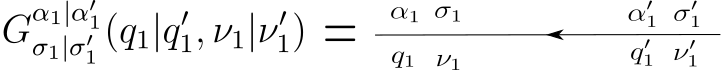
\includegraphics[width=0.75\textwidth]{propagator}
	\caption{Propagator line}
	\label{fig:prop}
\end{figure}



\subsection*{Frequency \& momentum conservation}
The fact that the propagator conserves energy and momentum (due to time- or, given the case, space-translation invariance) translates to the Green's functions being diagonal in frequency and momentum space, respectively.
\begin{align}
\text{Time trans. inv: } &G(t|t') = G(t-t')\\ &\Rightarrow G^{\alpha_1|\alpha'_1}_{\sigma_1|\sigma'_1}(q_1|q'_1, \nu_1| \nu'_1) = 2\pi i \delta(\nu_1-\nu'_1)G^{\alpha_1|\alpha'_1}_{\sigma_1|\sigma'_1}(q_1|q'_1, \nu_1)\\
\text{Space trans. inv: } &G(x|x') = G(x-x')\\ &\Rightarrow G^{\alpha_1|\alpha'_1}_{\sigma_1|\sigma'_1}(q_1|q'_1, \nu_1| \nu'_1) = 2\pi i \delta(q_1-q'_1)G^{\alpha_1|\alpha'_1}_{\sigma_1|\sigma'_1}(q_1, \nu_1| \nu'_1)\\
\text{Both: } &G(t|t', x|x') = G(t-t',x-x')\\ &\Rightarrow
(2\pi i)^2 \delta(q_1-q'_1)\delta(\nu_1-\nu'_1)G^{\alpha_1|\alpha'_1}_{\sigma_1|\sigma'_1}(q_1, \nu_1)
\end{align}
For this compendium we will assume time-invariance for all formulas but, since not all models will be translational invariant, we will not assume that symmetry.

\subsection*{Spin conservation}
Spin conservation leads to the Green's function begin diagonal in the finite dimensional spin-space (hence a Kronecker's instead of a Dirac's delta).
\begin{equation}
G_{\sigma_1|\sigma'_1} = \delta_{\sigma_1 \sigma'_1}G_{\sigma_1}
\end{equation}

\subsection*{Causality}
Causality in the Keldysh formalism translates to:
\begin{equation}
G^{1|1} = 0
\end{equation}

\subsection*{Complex conjugation}
Complex conjugation of the Green's function leads to the following equation:
\begin{equation}
\left[ G^{\alpha_1|\alpha'_1}_{\sigma_1}\right]^* = (-1)^{1+\alpha_1+\alpha'_1}G^{\alpha'_1|\alpha_1}_{\sigma_1}
\end{equation}
This means, effectively, that the direction of time is inverted (notice the flip in Keldysh indices).


\section*{Independent components of the single particle Green's function}
Within the Keldysh formalism, the propagator has three different non-zero components. Due to their analytical properties (considered as functions of a complex time variable $t\in \mathbb{C}$), these are called \textit{retarded}, \textit{advanced}, and \textit{Keldysh} components. They are defined as follows:
\begin{equation}
R \defeq G^R = G^{2|1}  \hspace{0.7cm} A \defeq G^A = G^{1|2}\hspace{0.7cm} K \defeq G^K = G^{2|2}
\end{equation}
The components, thanks to the general property of the Green's function under conjugation, follow the following two relations:

\begin{equation}
\left[R\right]^* = A \hspace{0.7cm} \left[K\right]^* = -K
\end{equation}
Hence, $K$ is purely imaginary and there are only \textit{two} independent Keldysh components for the propagator, which we choose to be $R$ and $K$.

One can accommodate the components of the Green's function in a matrix, using the $\alpha_1|\alpha'_1$ as row and column indices:

\begin{equation}
G^{\alpha_1|\alpha'_1}_{\sigma_1} =
\begin{pmatrix}
G^{1|1} & G^{1|2} \\
G^{2|1} & G^{2|2}
\end{pmatrix}_{\sigma_1|\sigma_1} = \begin{pmatrix}
0 & A \\ R & K
\end{pmatrix}_{\sigma_1|\sigma_1}
\end{equation}


\section*{General properties of the four-point vertex $\Gamma$}

\begin{equation}
    \Gamma = \Gamma_{1'2'|12} = \Gamma_{\sigma_1'\sigma_2'|\sigma_1\sigma_2}^{\alpha_1'\alpha_2'|\alpha_1\alpha_2}(q_1'q_2'|q_1q_2, \nu_1'\nu_2'|\nu_1\nu_2)
\end{equation}
\begin{figure}[H]
\centering
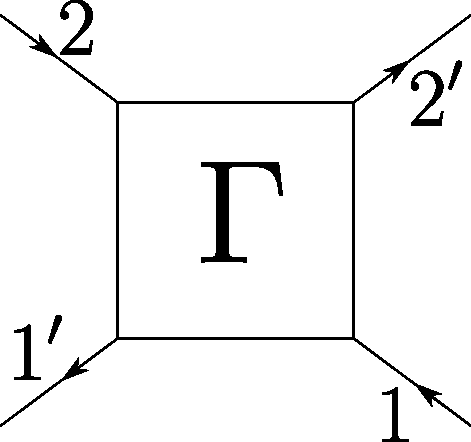
\includegraphics[scale=0.65]{vertex.pdf}
\caption{Convention for the vertex}
\label{fig:vertex}
\end{figure}
The Keldysh indices take values in the set $\{1,2\}$, with the convention $1 = q$ and $2=c$, where in some texts $c$ stands for 'classical component' and $q$ for 'quantum component'.
\subsection*{Spin conservation:}
Spin conservation: $\sigma_{1}^\prime + \sigma_{2}^\prime = \sigma_1 + \sigma_2$
\\
Overall spin conservation of the vertex dictates that there are two different cases:
\subsubsection*{All spins equal}
Sum of the incoming (or outgoing) spins equals either $-1$ or 1: 
$\Gamma = \Gamma_{\sigma\sigma|\sigma\sigma}$
\subsubsection*{Incoming spins reversed}
Sum of incoming spins equals 0: 
$\Gamma = \Gamma_{\sigma\overline{\sigma}|\sigma\overline{\sigma}}$ or $\Gamma = \Gamma_{\sigma\overline{\sigma}|\overline{\sigma}\sigma}$
These last two cases can be linked through a spin-inversion transformation and, hence, aren't considered to be (computationally) different, although they represent distinct physical processes.

\subsection*{Frequency conservation:}
Conservation of momentum implies that one of the frequencies, conventionally chosen to be $\nu_2$, will be dependent on the other three.
\begin{align}
    \nu_{1}^\prime + \nu_{2}^\prime &= \nu_1 + \nu_2  \\
    \implies \nu_2 &= \nu_{1}^\prime + \nu_{2}^\prime -\nu_1
\end{align}
Hence, we will omit $\nu_{2}$ altogether from all formulas it would have appeared in.

\subsection*{Causality:}
Causality, in the Keldysh formalism, translates to $\Gamma^{22|22} = 0$ always.

\subsection*{Particle exchange and complex conjugation:}
Here is how the vertex components are related under particle exchange:
\begin{align}
&\Gamma_{\sigma_2'\sigma_1'|\sigma_1\sigma_2}^{\alpha_2'\alpha_1'|\alpha_1\alpha_2}(q_2'q_1'|q_1q_2, \nu_2'\nu_1'|\nu_1\nu_2) \\
&= \Gamma_{\sigma_1'\sigma_2'|\sigma_2\sigma_1}^{\alpha_1'\alpha_2'|\alpha_2\alpha_1}(q_1'q_2'|q_2q_1, \nu_1'\nu_2'|\nu_2\nu_1) \\
&= - \Gamma_{\sigma_2'\sigma_1'|\sigma_2\sigma_1}^{\alpha_2'\alpha_1'|\alpha_2\alpha_1}(q_2'q_1'|q_2q_1, \nu_2'\nu_1'|\nu_2\nu_1) \\
&= - \Gamma_{\sigma_1'\sigma_2'|\sigma_1\sigma_2}^{\alpha_1'\alpha_2'|\alpha_1\alpha_2}(q_1'q_2'|q_1q_2, \nu_1'\nu_2'|\nu_1\nu_2)
\end{align}
And under complex conjugation:
\begin{multline}
\left[ \Gamma_{\sigma_1'\sigma_2'|\sigma_1\sigma_2}^{\alpha_1'\alpha_2'|\alpha_1\alpha_2}(q_1'q_2'|q_1q_2, \nu_1'\nu_2'|\nu_1\nu_2) \right]^* \\ =
(-1)^{(1+\alpha_1'+\alpha_2'+\alpha_1+\alpha_2)} \Gamma_{\sigma_1\sigma_2|\sigma_1'\sigma_2'}^{\alpha_1\alpha_2|\alpha_1'\alpha_2'}(q_1q_2|q_1'q_2', \nu_1\nu_2|\nu_1'\nu_2')
\end{multline}

\subsection*{Channel decomposition \& reducibility}
In the mfRG formalism we have that the full vertex can be written as the sum of the irreducible part $R = \Gamma_0 + \mathcal{O}(u^4)$ and reducible contributions $\gamma_r$ in three channels: $r=a$ for \textit{anti-parallel}, $r=p$ for \textit{parallel} and $r=t$ for \textit{transverse}. These names allude to the relation of the cut propagator lines have, were one to make a diagram disconnected. Since any reducible diagram can only belong to one of these classes, one can then write the following equation for the full vertex:
\begin{equation}
	\Gamma = \Gamma_0 + \sum_r \gamma_r = \Gamma_0 + \gamma_a + \gamma_p + \gamma_t
	\label{eq:simpleGammaDef}
\end{equation}

Including the spin and Keldysh indices, (but omitting the frequency and momentum dependencies) Eq. \eqref{eq:simpleGammaDef} becomes
\begin{equation}
	\Gamma_{\sigma_1'\sigma_2'|\sigma_1\sigma_2}^{\alpha_1'\alpha_2'|\alpha_1\alpha_2} \eqdef \left[\Gamma_0 \right]_{\sigma_1'\sigma_2'|\sigma_1\sigma_2}^{\alpha_1'\alpha_2'|\alpha_1\alpha_2} + \left[\gamma_a \right]_{\sigma_1'\sigma_2'|\sigma_1\sigma_2}^{\alpha_1'\alpha_2'|\alpha_1\alpha_2}\left[\gamma_p \right]_{\sigma_1'\sigma_2'|\sigma_1\sigma_2}^{\alpha_1'\alpha_2'|\alpha_1\alpha_2}\left[\gamma_t \right]_{\sigma_1'\sigma_2'|\sigma_1\sigma_2}^{\alpha_1'\alpha_2'|\alpha_1\alpha_2},
\end{equation}
where we introduce the notation $\left[\Gamma_0 \right]_{\sigma_1'\sigma_2'|\sigma_1\sigma_2}^{\alpha_1'\alpha_2'|\alpha_1\alpha_2}$ to imply the fact that the bare vertex, although trivial in frequency and momentum, has a non-trivial spin and Keldysh structure.

This structure is as follows \cite{PhysRevB.81.195109}:

\begin{equation}
	\left[\Gamma_0 \right]_{\sigma_1'\sigma_2'|\sigma_1\sigma_2}^{\alpha_1'\alpha_2'|\alpha_1\alpha_2} = \begin{cases}
	\frac{1}{2} \left[\Gamma_0 \right]_{\sigma_1'\sigma_2'|\sigma_1\sigma_2} \hspace{0.7cm}\text{if } \alpha_1'+\alpha_2' + \alpha_1+\alpha_2 \text{ is odd,} \\
	0, \text{ else,}
	\end{cases}
	\label{eq:defGamma0withKeldysh}
\end{equation}

with 

\begin{equation}
\left[\Gamma_0 \right]_{\sigma_1'\sigma_2'|\sigma_1\sigma_2} = \begin{cases}
U, \text{ if } \sigma_1'=\sigma_1= \overline{\sigma}'_2=\overline{\sigma}_2, \\
-U, \text{ if } \sigma_1'=\overline{\sigma}_1= \overline{\sigma}'_2=\sigma_2, \\
0, \text{ else.}
\end{cases}
\label{eq:defGamma0withourKeldysh}
\end{equation}

The reducibility of the diagrams then gives rise to the ``bubble'' objects, $\Pi_r$, which are the pair of propagators that, should they be cut, would disconnect the diagram. These pairs of propagators effectively carry a (bosonic) transfer frequency between the two sides of the bubble. Knowing this, we can tailor an explicit frequency dependence that highlights and exploits this fact, in order to then simplify calculations. Hence, we introduce the following structures:

\begin{figure}[ht]
    \centering
    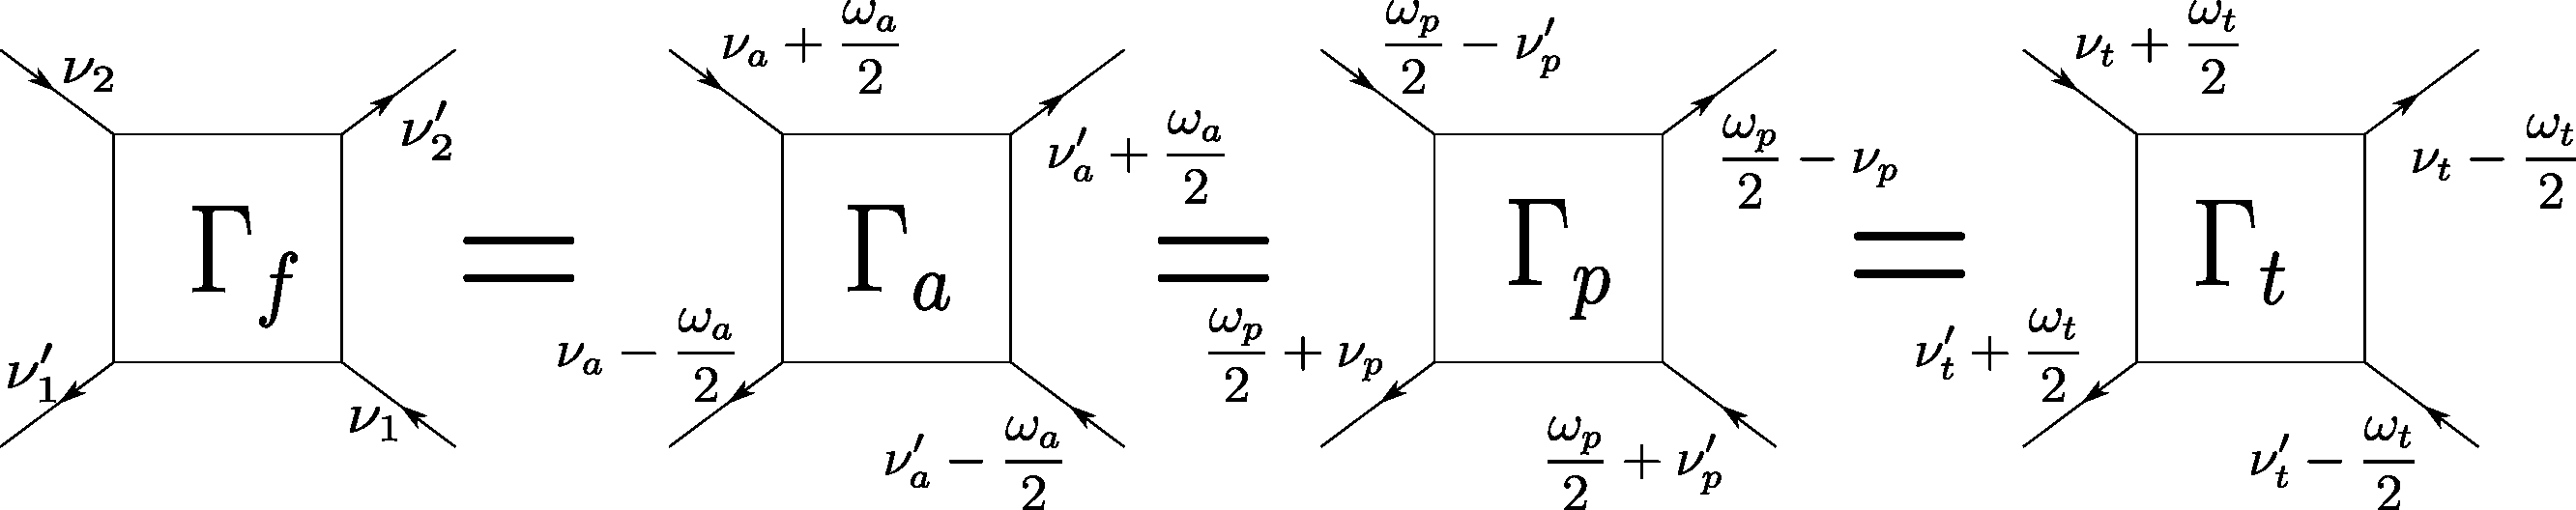
\includegraphics[width=\linewidth]{figures/channels_with_labels.pdf}
    \caption{Convention for the introduction of channel-specific frequencies}
    \label{fig:channels}
\end{figure}
In this notation we explicitly describe the full vertex function $\Gamma$, which is naturally a function of three arguments, as slight variations that depend on the convention for the respective channel:
\begin{align}
 \Gamma_f(\nu_1', \nu_2', \nu_1) &\hspace{0.7cm} \Gamma_a(\omega_a, \nu_a, \nu_a') \label{eq:vertexParam1}\\
 \Gamma_p(\omega_p, \nu_p, \nu_p') &\hspace{0.7cm} \Gamma_t(\omega_t, \nu_t, \nu_t')
 \label{eq:vertexParam2}
\end{align} 
This means that all $\Gamma_r$ represent the same object, namely the full vertex, but each instantiation receives the arguments $\omega_r$, $\nu_r$ and $\nu'_r$, the bosonic and the two fermionic frequencies (or all three fermionic frequencies, in the case of $r=f$), already expressed in the channel's natural parametrization. This clarification is important since these objects are fundamentally different from the notationally-similar $\gamma_r$, which are the reducible vertices in the $r$-channel.

The frequencies in Fig. \ref{fig:channels} lead then to the following conversion rules between the channels, where the conventional vertex depicted in Fig. \ref{fig:vertex} is referred to as the 'fermionic' vertex, $\Gamma_f$:

\subsubsection*{a-channel}
From and to the fermionic channel:
\begin{align}
    \left.\begin{array}{r@{\mskip\thickmuskip}l}
    \nu_{1'} &= \nu_a - \frac{\omega_a}{2} \\
    \nu_{2'} &= \nu'_a + \frac{\omega_a}{2} \\
    \nu_{1 } &= \nu'_a - \frac{\omega_a}{2} \\
  \end{array} \right\}
  \quad \implies \quad
  \left\{\begin{array}{l@{\mskip\thickmuskip}l}
    \omega_a &= \nu_{2} - \nu_{1'} = \nu_{2'} - \nu_{1}\\
    \nu_a    &= \frac{1}{2}\left(2\nu_{1'}+\nu_{2'}-\nu_{1}\right) \\
    \nu'_a   &= \frac{1}{2}\left(\nu_{2'} + \nu_{1}\right)\\
  \end{array}\right.
  \label{eq:AtoF}
\end{align}

And from any other channel to the a-channel:
\begin{align}
    \begin{array}{r@{\mskip\thickmuskip}l}
    \omega_a &= \omega_a\\
    \nu_a  &= \nu_a \\
    \nu'_a &= \nu'_a\\
  \end{array}
  \quad  \begin{array}{r@{\mskip\thickmuskip}l}
    \omega_a &= -\nu_p-\nu'_p\\
    \nu_a  &= \frac{\omega_p+\nu_p-\nu'_p}{2}\\
    \nu'_a &= \frac{\omega_p-\nu_p+\nu'_p}{2}\\
  \end{array} \quad
  \begin{array}{r@{\mskip\thickmuskip}l}
    \omega_a &= \nu_t-\nu'_t\\
    \nu_a  &= \frac{ \omega_t+\nu_t+\nu'_t}{2}\\
    \nu'_a &= \frac{-\omega_t+\nu_t+\nu'_t}{2}\\
  \end{array}
  \label{eq:AtoAll}
\end{align}


\subsubsection*{p-channel}
From and to the fermionic channel:
\begin{align}
    \left.\begin{array}{r@{\mskip\thickmuskip}l}
    \nu_{1'} &= \frac{\omega_p}{2} + \nu_p \\
    \nu_{2'} &= \frac{\omega_p}{2} - \nu_p \\
    \nu_{1}  &= \frac{\omega_p}{2} + \nu'_p\\
  \end{array} \right\}
  \quad \implies \quad
  \left\{\begin{array}{l@{\mskip\thickmuskip}l}
    \omega_p &= \nu_{1'} + \nu_{2'} = \nu_{1} + \nu_{2}\\
    \nu_p    &= \frac{1}{2}\left(\nu_{1'}-\nu_{2'}\right) \\
    \nu'_p   &= \frac{1}{2}\left(2\nu_{1}-\nu_{1'}-\nu_{2'}\right)\\
  \end{array}\right.
  \label{eq:PtoF}
\end{align}

And from any other channel to the p-channel:
\begin{align}
    \begin{array}{r@{\mskip\thickmuskip}l}
    \omega_p &= \nu_a+\nu'_a\\
    \nu_p  &= \frac{-\omega_a+\nu_a-\nu'_a}{2}\\
    \nu'_p &= \frac{-\omega_a-\nu_a+\nu'_a}{2}\\
  \end{array}
  \quad  \begin{array}{r@{\mskip\thickmuskip}l}
    \omega_p &= \omega_p\\
    \nu_p  &= \nu_p \\
    \nu'_p &= \nu'_p\\
  \end{array} \quad
  \begin{array}{r@{\mskip\thickmuskip}l}
    \omega_p &= \nu_t+\nu'_t\\
    \nu_p &= \frac{ \omega_t-\nu_t+\nu'_t}{2}\\
    \nu'_p &= \frac{-\omega_t-\nu_t+\nu'_t}{2}\\
  \end{array}
  \label{eq:PtoAll}
\end{align}

\subsubsection*{t-channel}
From and to the fermionic channel
\begin{align}
    \left.\begin{array}{r@{\mskip\thickmuskip}l}
    \nu_{1'} &= \nu'_t + \frac{\omega_t}{2} \\
    \nu_{2'} &= \nu_t  - \frac{\omega_t}{2} \\
    \nu_{1 } &= \nu'_t - \frac{\omega_t}{2} \\
  \end{array} \right\}
  \quad \implies \quad
  \left\{\begin{array}{l@{\mskip\thickmuskip}l}
    \omega_t &= \nu_{1'} - \nu_{1} = \nu_{2} - \nu_{2'}\\
    \nu_t    &= \frac{1}{2}\left(2\nu_{2'}+\nu_{1'}-\nu_{1}\right) \\
    \nu'_t   &= \frac{1}{2}\left(\nu_{1'} +\nu_{1}\right)\\
  \end{array}\right.
  \label{eq:TtoF}
\end{align}


And from any other channel to the t-channel:
\begin{align}
    \begin{array}{r@{\mskip\thickmuskip}l}
    \omega_t &= \nu_a-\nu'_a\\
    \nu_t  &= \frac{ \omega_a+\nu_a+\nu'_a}{2}\\
    \nu'_t &= \frac{-\omega_a+\nu_a+\nu'_a}{2}\\
  \end{array}
  \quad  \begin{array}{r@{\mskip\thickmuskip}l}
    \omega_t &= \nu_p-\nu'_p\\
    \nu_t  &= \frac{\omega_p-\nu_p-\nu'_p}{2}\\
    \nu'_t &= \frac{\omega_p+\nu_p+\nu'_p}{2}\\
  \end{array} \quad
  \begin{array}{r@{\mskip\thickmuskip}l}
    \omega_t &= \omega_t\\
    \nu_t  &= \nu_t \\
    \nu'_t &= \nu'_t\\
  \end{array}
  \label{eq:TtoAll}
\end{align}





\section*{Transformations}
Define the following transformations for the full vertex:
\subsection*{Spin flip}
\begin{equation}
T_S \Gamma^{\alpha_1'\alpha_2'|\alpha_1\alpha_2}_{\sigma_1'\sigma_2'|\sigma_1\sigma_2} (q_1'q_2'|q_1q_2, \nu_1'\nu_2'|\nu_1\nu_2) = \Gamma^{\alpha_1'\alpha_2'|\alpha_1\alpha_2}_{\bar{\sigma}_1'\bar{\sigma}_2'|\bar{\sigma}_1\bar{\sigma}_2} (q_1'q_2'|q_1q_2, \nu_1'\nu_2'|\nu_1\nu_2)
\end{equation}

\subsection*{Exchange symmetries}
Exchange of the Keldysh and spin indices of the incoming ($T_1$), outgoing ($T_2$) and incoming and outgoing ($T_3$) legs lead to the following vertex-internal dependencies:
\subsubsection*{Incoming legs exchange - $T_1$}
\begin{align}
    T_1 \left( \Gamma_{\sigma_1'\sigma_2'|\sigma_1\sigma_2}^{\alpha_1'\alpha_2'|\alpha_1\alpha_2}(q_1'q_2'|q_1q_2, \nu_1'\nu_2'|\nu_1\nu_2) \right) &= \Gamma_{\sigma_1'\sigma_2'|\sigma_2\sigma_1}^{\alpha_1'\alpha_2'|\alpha_2\alpha_1}(q_1'q_2'|q_1q_2, \nu_1'\nu_2'|\nu_1\nu_2)\\
    &= -\Gamma_{\sigma_1'\sigma_2'|\sigma_1\sigma_2}^{\alpha_1'\alpha_2'|\alpha_1\alpha_2}(q_1'q_2'|q_2q_1, \nu_1'\nu_2'|\nu_2\nu_1)
    \label{eq:t1}
\end{align}

\subsubsection*{Outgoing legs exchange - $T_2$}
\begin{align}
    T_2 \left( \Gamma_{\sigma_1'\sigma_2'|\sigma_1\sigma_2}^{\alpha_1'\alpha_2'|\alpha_1\alpha_2}(q_1'q_2'|q_1q_2, \nu_1'\nu_2'|\nu_1\nu_2) \right) &= \Gamma_{\sigma_2'\sigma_1'|\sigma_1\sigma_2}^{\alpha_2'\alpha_1'|\alpha_1\alpha_2}(q_1'q_2'|q_1q_2, \nu_1'\nu_2'|\nu_1\nu_2)\\
    &= -\Gamma_{\sigma_1'\sigma_2'|\sigma_1\sigma_2}^{\alpha_1'\alpha_2'|\alpha_1\alpha_2}(q_2'q_1'|q_1q_2, \nu_2'\nu_1'|\nu_1\nu_2)
    \label{eq:t2}
\end{align}

\subsubsection*{Incoming and outgoing legs exchange - $T_3$}
\begin{align}
    T_3 \left( \Gamma_{\sigma_1'\sigma_2'|\sigma_1\sigma_2}^{\alpha_1'\alpha_2'|\alpha_1\alpha_2}(q_1'q_2'|q_1q_2, \nu_1'\nu_2'|\nu_1\nu_2) \right) &= \Gamma_{\sigma_2'\sigma_1'|\sigma_2\sigma_1}^{\alpha_2'\alpha_1'|\alpha_2\alpha_1}(q_1'q_2'|q_1q_2, \nu_1'\nu_2'|\nu_1\nu_2)\\
    &= \Gamma_{\sigma_1'\sigma_2'|\sigma_1\sigma_2}^{\alpha_1'\alpha_2'|\alpha_1\alpha_2}(q_2'q_1'|q_2q_1, \nu_2'\nu_1'|\nu_2\nu_1)
    \label{eq:t3}
\end{align}

\subsubsection*{Complex conjugation (exchange of incoming and outgoing legs) - $T_C$}
\begin{align}
    T_C \large( \Gamma_{\sigma_1'\sigma_2'|\sigma_1\sigma_2}^{\alpha_1'\alpha_2'|\alpha_1\alpha_2}&(q_1'q_2'|q_1q_2, \nu_1'\nu_2'|\nu_1\nu_2) \large) = \Gamma_{\sigma_1\sigma_2|\sigma_1'\sigma_2'}^{\alpha_1\alpha_2|\alpha_1'\alpha_2'}(q_1'q_2'|q_1q_2, \nu_1'\nu_2'|\nu_1\nu_2)\\
    &=(-1)^{1+\alpha_1+\alpha_2+\alpha_1'+\alpha_2'}[ \Gamma_{\sigma_1'\sigma_2'|\sigma_1\sigma_2}^{\alpha_1'\alpha_2'|\alpha_1\alpha_2}(q_1q_2|q_1'q_2', \nu_1\nu_2|\nu_1'\nu_2')]^*
    \label{eq:tc}
\end{align}

Notice the $T_i$ transformations ($i\in \{1,2,3\}$) form a group which is isomorphic to the Klein group (every element has order 2 and $(T_i)^{-1} = T_i$). This fact, in combination with the action of $T_C$, the equations that define the multiplication map of the ``expanded'' group are:

\begin{align}
    \begin{array}{r@{\mskip\thickmuskip}l}
    T_1T_2 &= T_3\\
    T_2T_1 &= T_3
  \end{array} 
  \quad  \quad
  \begin{array}{l@{\mskip\thickmuskip}l}
    T_1T_C &= T_CT_2 \\
    T_C &= T_1T_CT_2 = T_2T_CT_1
  \end{array}
    \quad  \quad
  \begin{array}{l@{\mskip\thickmuskip}l}
  T_3T_C &= T_CT_3 \\
   & 
  \end{array}
\end{align}

As much as one would like the above table to be applicable to the channel decomposition of the vertex, this is simply not the case. Notice that the $T_1$ and $T_2$ symmetries exchange roles of corner-opposite legs of a diagram, which, when looked at in detail, means that the $a$ and $t$-channels get mapped into one another under these transformations. An exhaustive table of the cases will be presented after the following analysis of independent spin and Keldysh components in the vertex, since this work makes the other job much easier. 

\section*{Independent spin and Keldysh components}

The reducible part of the vertex in each channel can be decomposed into four diagrammatic classes:
\begin{align*}
\gamma_r (\omega_r, \nu_r, \nu_r^\prime) = \K1^r (\omega_r) + \K2^r (\omega_r, \nu_r) + \Kbar2^r (\omega_r, \nu_r^\prime) + \K3^r (\omega_r, \nu_r, \nu_r^\prime)
\end{align*}
\\
\textbf{Keldysh components which are equal due to diagrammatic structure of $\K1$, $\K2$, $\K3$}

Class $\K1$:
\begin{align*}
(\Ka1)\al121210 &= (\Ka1)\al121264 = (\Ka1)\al121273 = (\Ka1)\al121285 \\
(\Kp1)\al121210 &= (\Kp1)\al121280 = (\Kp1)\al121215 = (\Kp1)\al121285 \\
(\Kt1)\al121210 &= (\Kt1)\al121263 = (\Kt1)\al121274 = (\Kt1)\al121285 
\end{align*}

Class $\K2$, $\Kbar2$:
\begin{align*}
(\Ka2)\al121210 &= (\Ka2)\al121273 \,, \quad
(\Kabar2)\al121210 = (\Kabar2)\al121264 \\
(\Kp1)\al121210 &= (\Kp1)\al121215 \,, \quad
(\Kpbar1)\al121210 = (\Kpbar1)\al121280 \\
(\Kt2)\al121210 &= (\Kt2)\al121263 \,, \quad
(\Ktbar2)\al121210 = (\Ktbar2)\al121274
\end{align*}
\\
\\
The diagrammatic classes $\K1$, $\K2$, $\Kbar2$, $\K3$ behave differently under particle exchange and complex conjugation (also depending on the spin configuration), as elaborated further on. Here the multi-index notation $(1^\prime 2^\prime | 12)$ stands for Keldysh index, frequency, momentum. 

\subsection*{Equal spins $\sigma\sigma|\sigma\sigma$}

\textbf{Symmetries under particle exchange, complex conjugation}

Class $\K1$:
\begin{itemize}
	\item particle exchange:
	\begin{itemize}
		\item
		channels $a$, $t$:
		\begin{align*}
		\Ka1(1^\prime 2^\prime|12) &= -\Kt1(1^\prime 2^\prime|21) 
		\quad \Rightarrow \quad
		(\Ka1)\al121210 = T_1 (\Kt1)\al122110
		\\
		&= -\Kt1(2^\prime 1^\prime|12) 
		\quad \Rightarrow \quad
		(\Ka1)\al121210 = T_2 (\Kt1)\al211210
		\\
		\Ka1(1^\prime 2^\prime|12) & = \Ka1(2^\prime 1^\prime|21) 
		\quad \Rightarrow \quad
		(\Ka1)\al121210 = T_3 (\Ka1)\al212110
		\\
		\Kt1(1^\prime 2^\prime|12) & = \Kt1(2^\prime 1^\prime|21) 
		\quad \Rightarrow \quad
		(\Kt1)\al121210 = T_3 (\Kt1)\al212110
		\end{align*}
		\item channel $p$:
		\begin{align*}
		\Kp1(1^\prime 2^\prime|12) & = -\Kp1(1^\prime 2^\prime|21) 
		\quad \Rightarrow \quad
		(\Kp1)\al121210 = T_1 (\Kp1)\al122110
		\\
		&= -\Kp1(2^\prime 1^\prime|12) 
		\quad \Rightarrow \quad
		(\Kp1)\al121210 = T_2 (\Kp1)\al211210
		\\
		&= \Kp1(2^\prime 1^\prime|21)
		\quad \Rightarrow \quad
		(\Kp1)\al121210 = T_3 (\Kp1)\al212110
		\end{align*}
	\end{itemize}
	\item complex conjugation:
	\begin{align*}
	\K1^r(1^\prime 2^\prime|12) = (-1)^{\sum_j (1+\alpha_j + \bar{\alpha}_j)} (\K1^r(12|1^\prime 2^\prime))^*
	\quad \Rightarrow \quad
	(\K1^r)\al121210 = T_C (\K1^r)\al121201
	\end{align*}
\end{itemize}

Class $\K2$, $\Kbar2$:
\begin{itemize}
	\item particle exchange:
	\begin{itemize}
		\item
		channels $a$, $t$:
		\begin{align*}
		\Ka2(1^\prime 2^\prime|12) &= -\Ktbar2(1^\prime 2^\prime|21) 
		\quad \Rightarrow \quad
		(\Ka2)\al121210 = T_1 (\Ktbar2)\al122110
		\\
		&= -\Kt2(2^\prime 1^\prime|12) 
		\quad \Rightarrow \quad
		(\Ka2)\al121210 = T_2 (\Kt2)\al211210
		\\
		\Ka2(1^\prime 2^\prime|12) & = \Kabar2(2^\prime 1^\prime|21) 
		\quad \Rightarrow \quad
		(\Ka2)\al121210 = T_3 (\Kabar2)\al212110
		\\
		\Kt2(1^\prime 2^\prime|12) & = \Ktbar2(2^\prime 1^\prime|21) 
		\quad \Rightarrow \quad
		(\Kt2)\al121210 = T_3 (\Ktbar2)\al212110
		\end{align*}
		\item channel $p$:
		\begin{align*}
		\Kp2(1^\prime 2^\prime|12) & = -\Kp2(1^\prime 2^\prime|21) 
		\quad \Rightarrow \quad
		(\Kp2)\al121210 = T_1 (\Kp2)\al122110
		\\
		&= -\Kp2(2^\prime 1^\prime|12) 
		\quad \Rightarrow \quad
		(\Kp2)\al121210 = T_2 (\Kp2)\al211210
		\\
		&= \Kp2(2^\prime 1^\prime|21)
		\quad \Rightarrow \quad
		(\Kp2)\al121210 = T_3 (\Kp2)\al212110
		\end{align*}
		(similarly for $\Kpbar2$)
	\end{itemize}
	\item complex conjugation:
	\begin{align*}
	\K2^{a,p}(1^\prime 2^\prime|12) = &(-1)^{1+\sum_j (\alpha_j + \bar{\alpha}_j)} (\Kbar2^{a,p}(12|1^\prime 2^\prime))^*
	\quad\\ &\Rightarrow \quad
	(\K2^{a,p})\al121210 = T_C (\Kbar2^{a,p})\al121201 \\
	\Kt2(1^\prime 2^\prime|12) = &(-1)^{1+\sum_j (\alpha_j + \bar{\alpha}_j)} (\Kt2(12|1^\prime 2^\prime))^*
	\quad\\ &\Rightarrow \quad
	(\Kt2)\al121210 = T_C (\Kt2)\al121201 \\
	\Ktbar2(1^\prime 2^\prime|12) = &(-1)^{1+\sum_j (\alpha_j + \bar{\alpha}_j)} (\Ktbar2(12|1^\prime 2^\prime))^*
	\quad\\ &\Rightarrow \quad
	(\Ktbar2)\al121210 = T_C (\Ktbar2)\al121201
	\end{align*}
\end{itemize}

\subsubsection*{Enumeration of the components}
To make the whole thing a little easier and be able to refer to the components of the vertex in a concrete and ``linear'' manner, we convert the indices $\alpha_1'\alpha_2'|\alpha_1\alpha_2$ to numbers in the set $\mathcal{N} := \{0, 1, \dots, 15\}$. The following formula does the trick:
\begin{align}
i_\mathcal{N} &= 2^3(\alpha_1'-1)+2^2(\alpha_2'-1)+2^1(\alpha_1-1)+2^0(\alpha_2-1)\\
&= 8(\alpha_1'-1)+4(\alpha_2'-1)+2\alpha_1-1)+(\alpha_2-1)
\end{align}

There's also an inverse function for this, which involves using both the $\operatorname{floor}$
and the $\operatorname{mod}$ functions:

\begin{align}
\alpha_2 &= \left\lfloor{\frac{(i_\mathcal{N}\operatorname{mod}2)}{1}  }\right\rfloor +1 =(i_\mathcal{N}\operatorname{mod}2) +1\\
\alpha_1 &= \left\lfloor{\frac{(i_\mathcal{N}\operatorname{mod}4)}{2}  }\right\rfloor +1 \\
\alpha_2' &= \left\lfloor{\frac{(i_\mathcal{N}\operatorname{mod}8)}{4}  }\right\rfloor +1 \\
\alpha_1' &= \left\lfloor{\frac{(i_\mathcal{N}\operatorname{mod}16)}{8}  }\right\rfloor +1 
\end{align}

We summarize the results of these functions for future reference:
\begin{align}
\begin{array}{r@{\mskip\thickmuskip}l}
11|11 &\longleftrightarrow 0 \\
11|12 &\longleftrightarrow 1 \\
11|21 &\longleftrightarrow 2 \\
11|22 &\longleftrightarrow 3 \\
\vspace{0.05cm}\\
12|11 &\longleftrightarrow 4 \\
12|12 &\longleftrightarrow 5 \\
12|21 &\longleftrightarrow 6 \\
12|22 &\longleftrightarrow 7
\end{array} 
\quad  \quad
\begin{array}{l@{\mskip\thickmuskip}l}
21|11 &\longleftrightarrow 8 \\
21|12 &\longleftrightarrow 9 \\
21|21 &\longleftrightarrow 10 \\
21|22 &\longleftrightarrow 11 \\
\vspace{0.05cm}\\
22|11 &\longleftrightarrow 12 \\
22|12 &\longleftrightarrow 13 \\
22|21 &\longleftrightarrow 14 \\
22|22 &\longleftrightarrow 15
\end{array}
\end{align}
This allows us to refer to the components in the matrix as i.e. ``the 7th component'', where now it's unambiguously clear that the element referred to is $\Gamma^{12|22}$.

The above numeration and transformation properties of the respective diagrammatic classes yield the following tables:


%\renewcommand{\tabcolsep}{4pt} 
\begin{table}[H]
	\renewcommand{\arraystretch}{1.2}
	\begin{tabular}{c|c||ccc||ccc||ccc}
		\multicolumn{2}{c||}{} &
		\multicolumn{3}{c||}{$\sigma\sigma|\sigma\sigma$} & 
		\multicolumn{3}{c}{$\sigma\bar\sigma|\sigma\bar\sigma$} & 
		\multicolumn{3}{c}{$\sigma\bar\sigma|\bar\sigma\sigma$} 
		\\ 
		\multicolumn{2}{c||}{} & 
		$\Ka1$ & $\Kp1$ & $\Kt1$ & 
		$\Ka1$ & $\Kp1$ & $\Kt1$ & 
		$\Ka1$ & $\Kp1$ & $\Kt1$  
		\\ \hline
		
		1111 & 0 & 
		0 & 0 & 0 & 
		0 & 0 & 0 &
		0 & 0 & 0 
		\\ %\hline
		1112 & 1 & 
		\Ba1 & \Bp1 & \Bt1 & 
		\bBa1 & \bBp1 & \bBt1 &
		$T_S T_2$\bBt1 & $T_1$\bBp1 & $T_S T_2$\bBa1 
		\\ %\hline
		1121 & 2 & 
		$T_3$\Ba1 & \Bp1 & $T_3$\Bt1 & 
		$T_S T_3$\bBa1 & \bBp1 & $T_S T_3$\bBt1 &
		$T_1$\bBt1 & $T_1$\bBp1 & $T_1$\bBa1
		\\ %\hline
		1122 & 3 & 
		\Ca1 & 0 & \Ct1 & 
		\bCa1 & 0 & \bCt1 &
		$T_1$\bCt1 & 0 & $T_1$\bCa1
		\\ %\hline
		\hline
		
		
		1211 & 4 & 
		$T_3$\Ba1 & $T_C$\Bp1 & \Bt1 & 
		$T_S T_3$\bBa1 & $T_C$\bBp1 & \bBt1 &
		$T_1$\bBt1 & $T_1 T_C$\bBp1 & $T_S T_2$\bBa1 
		\\ %\hline
		1212 & 5 & 
		\Ca1 & \Dp1 & 0 & 
		\bCa1 & \bDp1 & 0 &
		$T_1$\bCt1 & $T_1$\bDp1 & 0
		\\ %\hline
		1221 & 6 & 
		0 & \Dp1 & \Ct1 & 
		0 & \bDp1 & \bCt1 &
		0 & $T_1$\bDp1 & $T_1$\bCa1
		\\ %\hline
		1222 & 7 & 
		\Ba1 & $T_C$\Bp1 & $T_3$\Bt1 & 
		\bBa1 & $T_C$\bBp1 & $T_S T_3$\bBt1 &
		$T_S T_2$\bBt1 & $T_1 T_C$\bBp1 & $T_1$\bBa1
		\\ %\hline
		\hline
		
		
		2111 & 8 & 
		\Ba1 & $T_C$\Bp1 & $T_3$\Bt1 & 
		\bBa1 & $T_C$\bBp1 & $T_S T_3$\bBt1 &
		$T_S T_2$\bBt1 & $T_1 T_C$\bBp1 & $T_1$\bBa1
		\\ %\hline
		2112 & 9 & 
		0 & \Dp1 & \Ct1 & 
		0 & \bDp1 & \bCt1 &
		0 & $T_1$\bDp1 & $T_1$\bCa1
		\\ %\hline
		2121 & 10 & 
		\Ca1 & \Dp1 & 0 & 
		\bCa1 & \bDp1 & 0 &
		$T_1$\bCt1 & $T_1$\bDp1 & 0
		\\ %\hline
		2122 & 11 & 
		$T_3$\Ba1 & $T_C$\Bp1 & \Bt1 & 
		$T_S T_3$\bBa1 & $T_C$\bBp1 & \bBt1 &
		$T_1$\bBt1 & $T_1 T_C$\bBp1 & $T_S T_2$\bBa1 
		\\ %\hline
		\hline
		
		
		2211 & 12 & 
		\Ca1 & 0 & \Ct1 & 
		\bCa1 & 0 & \bCt1 &
		$T_1$\bCt1 & 0 & $T_1$\bCa1
		\\ %\hline
		2212 & 13 & 
		$T_3$\Ba1 & \Bp1 & $T_3$\Bt1 & 
		$T_S T_3$\bBa1 & \bBp1 & $T_S T_3$\bBt1 &
		$T_1$\bBt1 & $T_1$\bBp1 & $T_1$\bBa1
		\\ %\hline
		2221 & 14 & 
		\Ba1 & \Bp1 & \Bt1 & 
		\bBa1 & \bBp1 & \bBt1 &
		$T_S T_2$\bBt1 & $T_1$\bBp1 & $T_S T_2$\bBa1 
		\\ %\hline
		2222 & 15 & 
		0 & 0 & 0 & 
		0 & 0 & 0 &
		0 & 0 & 0
		\\ \hline
	\end{tabular}
\end{table}



\begin{table}[H]
	\renewcommand{\arraystretch}{1.2}
	\begin{tabular}{c|c||c|c|c|c|c|c}
		\multicolumn{2}{c||}{} &
		\multicolumn{6}{c}{$\sigma\sigma|\sigma\sigma$}
		\\
		\multicolumn{2}{c||}{} &
		$\Ka2$ & $\Kabar2$ & 
		$\Kp2$ & $\Kpbar2$ & 
		$\Kt2$ & $\Ktbar2$  
		\\ \hline
		
		1111 & 0 & 
		\Aa2 & $T_3$\Aa2 & 
		\Ap2 & $T_C$\Ap2 & 
		$T_2$\Aa2 & $T_1$\Aa2 
		\\ %\hline
		1112 & 1 & 
		\Ba2 & $T_3$\Ca2 & 
		\Bp2 & $T_C$\Cp2 & 
		$T_2$\Ba2 & $T_1$\Ca2 
		\\ %\hline
		1121 & 2 & 
		\Ca2 & $T_3$\Ba2 & 
		\Bp2 & $T_C T_3$\Cp2 & 
		$T_2$\Ca2 & $T_1$\Ba2 
		\\ %\hline
		1122 & 3 & 
		\Da2 & $T_3$\Da2 & 
		\Ap2 & 0 & 
		$T_2$\Da2 & $T_1$\Da2 
		\\ %\hline
		\hline
		
		
		1211 & 4 & 
		\Ca2 & $T_C$\Ba2 & 
		\Cp2 & $T_C$\Bp2 & 
		$T_C T_2$\Ba2 & $T_1$\Ca2 
		\\ %\hline
		1212 & 5 & 
		\Da2 & $T_C$\Da2 & 
		\Dp2 & $T_C$\Dp2 & 
		0 & $T_1$\Aa2 
		\\ %\hline
		1221 & 6 & 
		\Aa2 & 0 & 
		\Dp2 & $T_C T_3$\Dp2 & 
		$T_C T_2$\Da2 & $T_1$\Da2  
		\\ %\hline
		1222 & 7 & 
		\Ba2 & $T_3$\Fa2 & 
		\Cp2 & $T_C$\Fp2 & 
		$T_2$\Fa2 & $T_1$\Ba2
		\\ %\hline
		\hline
		
		
		2111 & 8 & 
		$T_C T_3$\Ba2 & $T_3$\Ca2 & 
		$T_3$\Cp2 & $T_C$\Bp2 & 
		$T_2$\Ca2 & $T_C T_1$\Ba2
		\\ %\hline
		2112 & 9 & 
		0 & $T_3$\Aa2 & 
		$T_3$\Dp2 & $T_C$\Dp2 & 
		$T_2$\Da2 & $T_C T_1$\Da2 
		\\ %\hline
		2121 & 10 & 
		$T_C T_3$\Da2 & $T_3$\Da2 & 
		$T_3$\Dp2 & $T_C T_3$\Dp2 & 
		$T_2$\Aa2 & 0 
		\\ %\hline
		2122 & 11 & 
		\Fa2 & $T_3$\Ba2 & 
		$T_3$\Cp2 & $T_C$\Fp2 & 
		$T_2$\Ba2 & $T_1$\Fa2 
		\\ %\hline
		\hline
		
		
		2211 & 12 & 
		$T_C T_3$\Da2 & $T_C$\Da2 & 
		0 & $T_C$\Ap2 & 
		$T_C T_2$\Da2 & $T_C T_1$\Da2 
		\\ %\hline
		2212 & 13 & 
		\Fa2 & $T_C$\Ba2 & 
		\Fp2 & $T_C$\Cp2 & 
		$T_2$\Fa2 & $T_C T_1$\Ba2 
		\\ %\hline
		2221 & 14 & 
		$T_C T_3$\Ba2 & $T_3$\Fa2 & 
		\Fp2 & $T_C T_3$\Cp2 & 
		$T_C T_2$\Ba2 & $T_1$\Fa2 
		\\ %\hline
		2222 & 15 & 
		0 & 0 & 0 & 0 & 0 & 0 
		\\ %\hline
		\hline
	\end{tabular}
\end{table}


\begin{table}[H]
	\renewcommand{\arraystretch}{1.2}
	\begin{tabular}{c|c||c|c|c|c|c|c}
		\multicolumn{2}{c||}{} &
		\multicolumn{6}{c}{$\sigma\bar\sigma|\sigma\bar\sigma$}
		\\
		\multicolumn{2}{c||}{} &
		$\Ka2$ & $\Kabar2$ & 
		$\Kp2$ & $\Kpbar2$ & 
		$\Kt2$ & $\Ktbar2$  
		\\ \hline
		
		1111 & 0 & 
		\bAa2 & $T_S T_3$\bAa2 & 
		\bAp2 & $T_C$\bAp2 & 
		\bAt2 & $T_S T_3$\bAt2 
		\\ %\hline
		1112 & 1 & 
		\bBa2 & $T_S T_3$\bCa2 & 
		\bBp2 & $T_C$\bCp2 & 
		\bBt2 & $T_S T_3$\bCt2 
		\\ %\hline
		1121 & 2 & 
		\bCa2 & $T_S T_3$\bBa2 & 
		\bBp2 & $T_S T_C T_3$\bCp2 & 
		\bCt2 & $T_S T_3$\bBt2 
		\\ %\hline
		1122 & 3 & 
		\bDa2 & $T_S T_3$\bDa2 & 
		\bAp2 & 0 & 
		\bDt2 & $T_S T_3$\bDt2 
		\\ %\hline
		\hline
		
		
		1211 & 4 & 
		\bCa2 & $T_C$\bBa2 & 
		\bCp2 & $T_C$\bBp2 & 
		$T_C$\bBt2 & $T_S T_3$\bCt2 
		\\ %\hline
		1212 & 5 & 
		\bDa2 & $T_C$\bDa2 & 
		\bDp2 & $T_C$\bDp2 & 
		0 & $T_S T_3$\bAt2 
		\\ %\hline
		1221 & 6 & 
		\bAa2 & 0 & 
		\bDp2 & $T_S T_C T_3$\bDp2 & 
		$T_C$\bDt2 & $T_S T_3$\bDt2  
		\\ %\hline
		1222 & 7 & 
		\bBa2 & $T_S T_3$\bFa2 & 
		\bCp2 & $T_C$\bFp2 & 
		\bFt2 & $T_S T_3$\bBt2
		\\ %\hline
		\hline
		
		
		2111 & 8 & 
		$T_S T_C T_3$\bBa2 & $T_S T_3$\bCa2 & 
		$T_S T_3$\bCp2 & $T_C$\bBp2 & 
		\bCt2 & $T_S T_C T_3$\bBt2
		\\ %\hline
		2112 & 9 & 
		0 & $T_S T_3$\bAa2 & 
		$T_S T_3$\bDp2 & $T_C$\bDp2 & 
		\bDt2 & $T_S T_C T_3$\bDt2 
		\\ %\hline
		2121 & 10 & 
		$T_S T_C T_3$\bDa2 & $T_S T_3$\bDa2 & 
		$T_S T_3$\bDp2 & $T_S T_C T_3$\bDp2 & 
		\bAt2 & 0 
		\\ %\hline
		2122 & 11 & 
		\bFa2 & $T_S T_3$\bBa2 & 
		$T_S T_3$\bCp2 & $T_C$\bFp2 & 
		\bBt2 & $T_S T_3$\bFt2 
		\\ %\hline
		\hline
		
		
		2211 & 12 & 
		$T_S T_C T_3$\bDa2 & $T_C$\bDa2 & 
		0 & $T_C$\bAp2 & 
		$T_C$\bDt2 & $T_S T_C T_3$\bDt2 
		\\ %\hline
		2212 & 13 & 
		\bFa2 & $T_C$\bBa2 & 
		\bFp2 & $T_C$\bCp2 & 
		\bFt2 & $T_S T_C T_3$\bBt2 
		\\ %\hline
		2221 & 14 & 
		$T_S T_C T_3$\bBa2 & $T_S T_3$\bFa2 & 
		\bFp2 & $T_S T_C T_3$\bCp2 & 
		$T_C$\bBt2 & $T_S T_3$\bFt2 
		\\ %\hline
		2222 & 15 & 
		0 & 0 & 0 & 0 & 0 & 0 
		\\ %\hline
		\hline
	\end{tabular}
\end{table}



\begin{table}[H]
	\renewcommand{\arraystretch}{1.2}
	\begin{tabular}{c|c||c|c|c|c|c|c}
		\multicolumn{2}{c||}{} &
		\multicolumn{6}{c}{$\sigma\bar\sigma|\bar\sigma\sigma$}
		\\
		\multicolumn{2}{c||}{} &
		$\Ka2$ & $\Kabar2$ & 
		$\Kp2$ & $\Kpbar2$ & 
		$\Kt2$ & $\Ktbar2$ 
		\\ \hline
		
		1111 & 0 & 
		$T_S T_2$\bAt2 & $T_1$\bAt2 & 
		$T_1$\bAp2 & $T_S T_C T_1$\bAp2 & 
		$T_S T_2$\bAa2 & $T_1$\bAa2 
		\\ %\hline
		1112 & 1 & 
		$T_S T_2$\bBt2 & $T_1$\bCt2 & 
		$T_1$\bBp2 & $T_S T_C T_1$\bCp2 & 
		$T_S T_2$\bBa2 & $T_1$\bCa2 
		\\ %\hline
		1121 & 2 & 
		$T_S T_2$\bCt2 & $T_1$\bBt2 & 
		$T_1$\bBp2 & $T_1 T_C$\bCp2 & 
		$T_S T_2$\bCa2 & $T_1$\bBa2 
		\\ %\hline
		1122 & 3 & 
		$T_S T_2$\bDt2 & $T_1$\bDt2 & 
		$T_1$\bAp2 & 0 & 
		$T_S T_2$\bDa2 & $T_1$\bDa2 
		\\ %\hline
		\hline
		
		
		1211 & 4 & 
		$T_S T_2$\bCt2 & $T_1 T_C$\bBt2 & 
		$T_1$\bCp2 & $T_1 T_C$\bBp2 & 
		$T_1 T_C$\bBa2 & $T_1$\bCa2 
		\\ %\hline
		1212 & 5 & 
		$T_S T_2$\bDt2 & $T_1 T_C$\bDt2 & 
		$T_1$\bDp2 & $T_S T_C T_1$\bDp2 & 
		0 & $T_1$\bAa2 
		\\ %\hline
		1221 & 6 & 
		$T_S T_2$\bAt2 & 0 & 
		$T_1$\bDp2 & $T_1 T_C$\bDp2 & 
		$T_1 T_C$\bDa2 & $T_1$\bDa2  
		\\ %\hline
		1222 & 7 & 
		$T_S T_2$\bBt2 & $T_1$\bFt2 & 
		$T_1$\bCp2 & $T_S T_C T_1$\bFp2 & 
		$T_S T_2$\bFa2 & $T_1$\bBa2
		\\ %\hline
		\hline
		
		
		2111 & 8 & 
		$T_S T_C T_1$\bBt2 & $T_1$\bCt2 & 
		$T_S T_2$\bCp2 & $T_1 T_C$\bBp2 & 
		$T_S T_2$\bCa2 & $T_S T_C T_1$\bBa2
		\\ %\hline
		2112 & 9 & 
		0 & $T_1$\bAt2 & 
		$T_S T_2$\bDp2 & $T_S T_C T_1$\bDp2 & 
		$T_S T_2$\bDa2 & $T_S T_C T_1$\bDa2 
		\\ %\hline
		2121 & 10 & 
		$T_S T_C T_1$\bDt2 & $T_1$\bDt2 & 
		$T_S T_2$\bDp2 & $T_1 T_C$\bDp2 & 
		$T_S T_2$\bAa2 & 0 
		\\ %\hline
		2122 & 11 & 
		$T_S T_2$\bFt2 & $T_1$\bBt2 & 
		$T_S T_2$\bCp2 & $T_S T_C T_1$\bFp2 & 
		$T_S T_2$\bBa2 & $T_1$\bFa2 
		\\ %\hline
		\hline
		
		
		2211 & 12 & 
		$T_S T_C T_1$\bDt2 & $T_1 T_C$\bDt2 & 
		0 & $T_S T_C T_1$\bAp2 & 
		$T_1 T_C$\bDa2 & $T_S T_C T_1$\bDa2 
		\\ %\hline
		2212 & 13 & 
		$T_S T_2$\bFt2 & $T_1 T_C$\bBt2 & 
		$T_1$\bFp2 & $T_S T_C T_1$\bCp2 & 
		$T_S T_2$\bFa2 & $T_S T_C T_1$\bBa2 
		\\ %\hline
		2221 & 14 & 
		$T_S T_C T_1$\bBt2 & $T_1$\bFt2 & 
		$T_1$\bFp2 & $T_1 T_C$\bCp2 & 
		$T_1 T_C$\bBa2 & $T_1$\bFa2 
		\\ %\hline
		2222 & 15 & 
		0 & 0 & 0 & 0 & 0 & 0 
		\\ %\hline
		\hline
	\end{tabular}
\end{table}


\renewcommand{\tabcolsep}{0.5pt}  % 2pt
\begin{table}[H]
	\renewcommand{\arraystretch}{1.2}
	\begin{tabular}{c|c||c|c|c||c|c|c||c|c|c}
		\multicolumn{2}{c||}{} &
		\multicolumn{3}{c||}{$\sigma\sigma|\sigma\sigma$} & 
		\multicolumn{3}{c}{$\sigma\bar\sigma|\sigma\bar\sigma$} & 
		\multicolumn{3}{c}{$\sigma\bar\sigma|\bar\sigma\sigma$} 
		\\ 
		\multicolumn{2}{c||}{} & 
		$\Ka3$ & $\Kp3$ & $\Kt3$ &
		$\Ka3$ & $\Kp3$ & $\Kt3$ &
		$\Ka3$ & $\Kp3$ & $\Kt3$ 
		\\ \hline
		
		1111 & 0 & 
		\Aa3 & \Ap3 & $T_2$\Aa3 &
		\bAa3 & \bAp3 & \bAt3 &
		$T_1$\bAt3 & $T_1$\bAp3 & $T_1$\bAa3
		\\ %\hline
		1112 & 1 & 
		\Ba3 & \Bp3 & $T_2$\Ba3 &
		\bBa3 & \bBp3 & \bBt3 &
		$T_S T_2$\bBt3 & $T_S T_2$\bBp3 & $T_S T_2$\bBa3
		\\ %\hline
		1121 & 2 & 
		$T_3$\Ba3 & $T_3$\Bp3 & $T_1$\Ba3 &
		$T_S T_3$\bBa3 & $T_S T_3$\bBp3 & $T_S T_3$\bBt3 &
		$T_1$\bBt3 & $T_1$\bBp3 & $T_1$\bBa3
		\\ %\hline
		1122 & 3 & 
		\Ca3 & \Cp3 & $T_2$\Ca3 &
		\bCa3 & \bCp3 & \bCt3 &
		$T_1$\bCt3 & $T_1$\bCp3 & $T_1$\bCa3
		\\ %\hline
		\hline
		
		
		1211 & 4 & 
		$T_C$\Ba3 & $T_C$\Bp3 & $T_1 T_C$\Ba3 &
		$T_C$\bBa3 & $T_C$\bBp3 & $T_C$\bBt3 &
		$T_1 T_C$\bBt3 & $T_1 T_C$\bBp3 & $T_1 T_C$\bBa3
		\\ %\hline
		1212 & 5 & 
		\Da3 & \Dp3 & \Dt3 &
		\bDa3 & \bDp3 & \bDt3 &
		$T_1$\bEt3 & $T_1$\bEp3 & $T_1$\bEa3
		\\ %\hline
		1221 & 6 & 
		$T_1$\Dt3 & $T_1$\Dp3 & $T_1$\Da3 &
		\bEa3 & \bEp3 & \bEt3 &
		$T_1$\bDt3 & $T_1$\bDp3 & $T_1$\bDa3
		\\ %\hline
		1222 & 7 & 
		\Fa3 & \Fp3 & $T_1$\Fa3 &
		\bFa3 & \bFp3 & \bFt3 &
		$T_1$\bFt3 & $T_1$\bFp3 & $T_1$\bFa3
		\\ %\hline
		\hline
		
		
		2111 & 8 & 
		$T_C T_3$\Ba3 & $T_C T_3$\Bp3 & $T_C T_1$\Ba3 &
		$T_S T_C T_3$\bBa3 & $T_S T_C T_3$\bBp3 & $T_S T_C T_3$\bBt3 &
		$T_S T_C T_1$\bBt3 & $T_S T_C T_1$\bBp3 & $T_S T_C T_1$\bBa3
		\\ %\hline
		2112 & 9 & 
		$T_2$\Dt3 & $T_2$\Dp3 & $T_2$\Da3 &
		$T_S T_3$\bEa3 & $T_S T_3$\bEp3 & $T_S T_3$\bEt3 & 
		$T_S T_2$\bDt3 & $T_S T_2$\bDp3 & $T_S T_2$\bDa3
		\\ %\hline
		2121 & 10 & 
		$T_3$\Da3 & $T_3$\Dp3 & $T_3$\Dt3 &
		$T_S T_3$\bDa3 & $T_S T_3$\bDp3 & $T_S T_3$\bDt3 & 
		$T_S T_2$\bEt3 & $T_S T_2$\bEp3 & $T_S T_2$\bEa3
		\\ %\hline
		2122 & 11 & 
		$T_3$\Fa3 & $T_3$\Fp3 & $T_2$\Fa3 &
		$T_S T_3$\bFa3 & $T_S T_3$\bFp3 & $T_S T_3$\bFt3 & 
		$T_S T_2$\bFt3 & $T_S T_2$\bFp3 & $T_S T_2$\bFa3
		\\ %\hline
		\hline
		
		
		2211 & 12 & 
		$T_C$\Ca3 & $T_C$\Cp3 & $T_1 T_C$\Ca3 &
		$T_C$\bCa3 & $T_C$\bCp3 & $T_C$\bCt3 &
		$T_1 T_C$\bCt3 & $T_1 T_C$\bCp3 & $T_1 T_C$\bCa3
		\\ %\hline
		2212 & 13 & 
		$T_C$\Fa3 & $T_C$\Fp3 & $T_2 T_C$\Fa3 &
		$T_C$\bFa3 & $T_C$\bFp3 & $T_C$\bFt3 &
		$T_S T_C T_1$\bFt3 & $T_S T_C T_1$\bFp3 & $T_S T_C T_1$\bFa3
		\\ %\hline
		2221 & 14 & 
		$T_C T_3$\Fa3 & $T_C T_3$\Fp3 & $T_C T_2$\Fa3 &
		$T_S T_C T_3$\bFa3 & $T_S T_C T_3$\bFp3 & $T_S T_C T_3$\bFt3 &
		$T_1 T_C$\bFt3 & $T_1 T_C$\bFp3 & $T_1 T_C$\bFa3
		\\ %\hline
		2222 & 15 & 
		0 & 0 & 0 &
		0 & 0 & 0 &
		0 & 0 & 0
		\\
		\hline
		
		
	\end{tabular}
\end{table}

\section*{General properties of the self energy $\Sigma$}
The self energy has similar symmetry properties as the propagator. Thus, the following diagrammatic representation:
\begin{figure}[h]
	\centering
	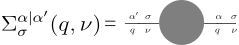
\includegraphics[width=0.75\textwidth]{self_energy}
\end{figure}


It also has two independent components, $\Sigma^R$, which it's conjugate is $\Sigma^A = \left[\Sigma^R\right]^*$ and $\Sigma^K$, which is anti-hermitian, i.e. $\left[\Sigma^K\right]^* = -\Sigma^K$. However, causality for the self-energy translates to $\Sigma^{2|2}=0$, such that it's Keldysh structure in matrix form reads
\begin{equation}
\Sigma^{\alpha'_1|\alpha_1}_{\sigma_1} =
\begin{pmatrix}
\Sigma^{1|1} & \Sigma^{1|2} \\
\Sigma^{2|1} & \Sigma^{2|2}
\end{pmatrix}_{\sigma_1|\sigma_1} = \begin{pmatrix}
\Sigma^K & \Sigma^R \\ \Sigma^A & 0
\end{pmatrix}_{\sigma_1|\sigma_1}
\end{equation}

\subsection*{Computing the self energy}
For computing the self energy, we take the contribution from all the $2n$-point vertices that we have (in our truncation only $\Gamma$, the four-point vertex, whose properties come in the next section) to the 2 point-vertex. Hence, we get the following equation:

\begin{align}
\Sigma^{\alpha_1'|\alpha_1}_{\sigma_1'|\sigma_{1}}(\nu_1'|\nu_1) &= \sum_{\sigma_2', \sigma_2}\sum_{\alpha_2', \alpha_2} \int \frac{\dd\nu_2'}{2\pi i} \frac{\dd\nu_2}{2\pi i} G^{\alpha_2|\alpha'_2}_{\sigma_2'|\sigma_2}(\nu_2| \nu_2') \Gamma_{\sigma_1'\sigma_2'|\sigma_1\sigma_2}^{\alpha_1'\alpha_2'|\alpha_1\alpha_2}(\nu_1', \nu_2'| \nu_1, \nu_2)
\label{eq:defSelfEnergy}
\end{align}
Using the fact that $G$ is diagonal in frequency and spin spaces, we can, through a Kronecker and a Dirac delta, get rid of the first sum as well as of one of the integrals. Hence, as mentioned above, $\Sigma$ inherits the same properties in frequency and spin spaces from $G$.

Simplifying Eq.~\eqref{eq:defSelfEnergy} according to this, one then obtains the actual formula to be used:
\begin{align}
\Sigma^{\alpha_1'|\alpha_1}_{\sigma_1}(\nu) &= \sum_{\sigma'} \sum_{\alpha_2', \alpha_2} \int \frac{\dd\nu'}{2\pi i} \Gamma_{\sigma\sigma'|\sigma\sigma'}^{\alpha_1'\alpha_2'|\alpha_1\alpha_2}(\nu, \nu'| \nu, \nu')G^{\alpha_2|\alpha'_2}_{\sigma'}(\nu')
\label{eq:actualSelfEnergy}
\end{align}

Since we'll be interested in a $\Lambda$-dependent RG-flow, we also include the case for $\dot{\Sigma}^\Lambda$, where now both $\Gamma \rightarrow \Gamma^\Lambda$ and $G \rightarrow G^\Lambda$ start to depend on the scale parameter $\Lambda$. 

\begin{align}
\dot{\Sigma}^{\alpha_1'|\alpha_1}_{\sigma_1}(\nu) &= \sum_{\sigma'} \sum_{\alpha_2', \alpha_2} \int \frac{\dd\nu'}{2\pi i}  \Gamma_{\sigma\sigma'|\sigma\sigma'}^{\alpha_1'\alpha_2'|\alpha_1\alpha_2}(\nu, \nu'| \nu, \nu')S^{\alpha_2|\alpha'_2}_{\sigma'}(\nu')\\
&= \sum_{\sigma'} \sum_{\alpha_2', \alpha_2} \int \frac{\dd\nu'}{2\pi i}  \left[\Gamma_f\right]_{\sigma\sigma'|\sigma\sigma'}^{\alpha_1'\alpha_2'|\alpha_1\alpha_2}(\nu, \nu', \nu)S^{\alpha_2|\alpha'_2}_{\sigma'}(\nu')
\label{eq:derivativeSelfEnergy}
\end{align}
Here we are using the notation introduced in Fig.\ref{fig:channels} and Eqs.\eqref{eq:vertexParam1} and \eqref{eq:vertexParam2} and the single-scale propagator $S^\Lambda \defeq \partial_\Lambda G|_{\Sigma =\text{ const.}}$. $S$ also has a Keldysh structure which is, unsurprisingly, exactly equal to the one of the propagator $G$. Note that it's important that we take $S$ for calculating $\Sigma$ in a first instance and not $\partial_\Lambda G = S + G\circ \dot{\Sigma}\circ G$, since the second term constitute corrections (of course this must be accounted somewhere, just not here).

Now, exploiting the fact that we only need two components of $\Sigma$ (namely $\Sigma^K=\Sigma^{1|1}$ and $\Sigma^R=\Sigma^{1|2}$), we write off the explicit contributions these receive:

\begin{align}
\begin{split}
\dot{\Sigma}^{1|1}_\sigma(\nu) =\dot{\Sigma}^K_\sigma(\nu) = \sum_{\sigma'}&\sum_{\alpha_2', \alpha_2}\int \frac{\dd\nu'}{2\pi i} \left[\Gamma_f\right]_{\sigma\sigma'|\sigma\sigma'}^{1\alpha_2'|1\alpha_2}(\nu, \nu', \nu)S^{\alpha_2|\alpha_2'}_{\sigma'}(\nu')
\end{split}\\
\begin{split}
= \sum_{\sigma'} \Bigl(
&\left[\Gamma_f\right]_{\sigma\sigma'|\sigma\sigma'}^{11|12}(\nu, \nu', \nu)S^R_{\sigma'}(\nu') +\\
&\left[\Gamma_f\right]_{\sigma\sigma'|\sigma\sigma'}^{12|11}(\nu, \nu', \nu)S^A_{\sigma'}(\nu') +\\
& \left[\Gamma_f\right]_{\sigma\sigma'|\sigma\sigma'}^{12|12}(\nu, \nu', \nu)S^K_{\sigma'}(\nu')\Bigr)
\end{split}\\
\begin{split}
= \sum_{\sigma'} \Bigl(
&\left[\Gamma_f\right]_{\sigma\sigma'|\sigma\sigma'}^{1}(\nu, \nu', \nu)S^R_{\sigma'}(\nu') +\\
&\left[\Gamma_f\right]_{\sigma\sigma'|\sigma\sigma'}^{4}(\nu, \nu', \nu)S^A_{\sigma'}(\nu') +\\
& \left[\Gamma_f\right]_{\sigma\sigma'|\sigma\sigma'}^{5}(\nu, \nu', \nu)S^K_{\sigma'}(\nu')\Bigr)
\label{eq:SigmaK}
\end{split}
\end{align}

\begin{align}
\begin{split}
\dot{\Sigma}^{1|2}_\sigma(\nu) =\dot{\Sigma}^R_\sigma(\nu) = \sum_{\sigma'}&\sum_{\alpha_2', \alpha_2}\int \frac{\dd\nu'}{2\pi i} \left[\Gamma_f\right]_{\sigma\sigma'|\sigma\sigma'}^{1\alpha_2'|2\alpha_2}(\nu, \nu', \nu)S^{\alpha_2|\alpha_2'}_{\sigma'}(\nu')
\end{split}\\
\begin{split}
= \sum_{\sigma'} \Bigl(
&\left[\Gamma_f\right]_{\sigma\sigma'|\sigma\sigma'}^{11|22}(\nu, \nu', \nu)S^R_{\sigma'}(\nu') +\\
&\left[\Gamma_f\right]_{\sigma\sigma'|\sigma\sigma'}^{12|21}(\nu, \nu', \nu)S^A_{\sigma'}(\nu') +\\
& \left[\Gamma_f\right]_{\sigma\sigma'|\sigma\sigma'}^{12|22}(\nu, \nu', \nu)S^K_{\sigma'}(\nu')\Bigr)
\end{split}\\
\begin{split}
= \sum_{\sigma'} \Bigl(
&\left[\Gamma_f\right]_{\sigma\sigma'|\sigma\sigma'}^{3}(\nu, \nu', \nu)S^R_{\sigma'}(\nu') +\\
&\left[\Gamma_f\right]_{\sigma\sigma'|\sigma\sigma'}^{6}(\nu, \nu', \nu)S^A_{\sigma'}(\nu') +\\
& \left[\Gamma_f\right]_{\sigma\sigma'|\sigma\sigma'}^{7}(\nu, \nu', \nu)S^K_{\sigma'}(\nu')\Bigr)
\end{split}
\label{eq:SigmaR}
\end{align}

At this point, one could be completely satisfied with Eqs. \eqref{eq:SigmaK} and \eqref{eq:SigmaR}. However, these make no use whatsoever of the channel decomposition, which does offer some computational advantages in performance and it yields possibilities to benchmark code segments.

Using Eqs.\eqref{eq:AtoF}, \eqref{eq:PtoF} and \eqref{eq:TtoF} to transform the fermionic frequencies to the corresponding frequencies of the respective channels, one obtains the following equation for $\dot{\Sigma}$, following Eq. \eqref{eq:derivativeSelfEnergy}.

\begin{align}
	\begin{split}
	\dot{\Sigma}^{\alpha_1'|\alpha_1}_\sigma (\nu) = \sum_{\sigma'} \sum_{\alpha_2', \alpha_2} \int \frac{\dd\nu'}{2\pi i} \Bigg( &\left[\Gamma_a\right]^{\alpha_1'\alpha_2'|\alpha_1\alpha_2}_{\sigma\sigma'|\sigma\sigma'}\left(\nu'-\nu, \frac{\nu+\nu'}{2}, \frac{\nu+\nu'}{2}\right) S^{\alpha_2|\alpha'_2}_{\sigma'}(\nu')\\
	+&\left[\Gamma_p\right]^{\alpha_1'\alpha_2'|\alpha_1\alpha_2}_{\sigma\sigma'|\sigma\sigma'}\left(\nu+\nu', \frac{\nu-\nu'}{2}, \frac{\nu-\nu'}{2}\right)
	S^{\alpha_2|\alpha'_2}_{\sigma'}(\nu') \\
	+&\left[\Gamma_t\right]^{\alpha_1'\alpha_2'|\alpha_1\alpha_2}_{\sigma\sigma'|\sigma\sigma'}\left(0, \nu', \nu \right) S^{\alpha_2|\alpha'_2}_{\sigma'}(\nu')\\
	+&\left[\Gamma_0\right]^{\alpha_1'\alpha_2'|\alpha_1\alpha_2}_{\sigma\sigma'|\sigma\sigma'} S^{\alpha_2|\alpha'_2}_{\sigma'}(\nu')\Bigg)\end{split}
	\label{eq:SigmaDotinChannels}
\end{align}

Notice that comparing results using Eqs. \eqref{eq:derivativeSelfEnergy} and \eqref{eq:SigmaDotinChannels} provides a computational consistency check that one can perform in order to check and verify that the frequency transformations between the fermionic and the $r$-channels is correctly implemented. Also, since the inputs are tailored to the way the vertices are parameterized, the computation of the self energy is slightly faster using the second formula.

A crucial remark that needs to be made at this point regarding the causality structure of the last term in Eq. \eqref{eq:SigmaDotinChannels}. According to Ref. \cite{kamenev_2011}, 
\begin{equation}
	G^R(t,t) + G^A(t,t) = 0.
	\label{eq:SameTimeSum}
\end{equation}

Eq. \ref{eq:SameTimeSum}, when converted to frequency space, takes the following form:
\begin{align}
\int \frac{\dd \nu}{2 \pi} \left( G^R(\nu) + G^A(\nu) \right) &= 0\\
\partial_\Lambda\Rightarrow \int \frac{\dd \nu}{2 \pi} \left( S^R(\nu) + S^A(\nu) \right) &= 0
\label{eq:SameTimeConstranit}
\end{align}

This same term is part of Eq. \eqref{eq:SigmaDotinChannels} for the case $\alpha_1=\alpha_1' = 1$, i.e. for contributions to $\Sigma^K$. If one \textit{only} writes the expansion of the sum for the last term of Eq. \eqref{eq:SigmaDotinChannels}, one obtains the following:
\begin{align}
	\left[\dot{\Sigma}^K_\sigma(\nu)\right]_0 = &\sum_{\sigma'} \int \frac{\dd \nu'}{2\pi i}\bigg(\left[\Gamma_0\right]^{11|12}_{\sigma\sigma'|\sigma\sigma'} S_{\sigma'}^R  
	+ \left[\Gamma_0\right]^{12|11}_{\sigma\sigma'|\sigma\sigma'} S_{\sigma'}^A  
	+\left[\Gamma_0\right]^{12|12}_{\sigma\sigma'|\sigma\sigma'} S_{\sigma'}^K  \bigg) \\
	\xRightarrow{Eq. \text{\eqref{eq:defGamma0withKeldysh}}} &\sum_{\sigma'} \int \frac{\dd \nu'}{2\pi i}\bigg(\left[\Gamma_0\right]_{\sigma\sigma'|\sigma\sigma'} S_{\sigma'}^R  
	+ \left[\Gamma_0\right]_{\sigma\sigma'|\sigma\sigma'} S_{\sigma'}^A \bigg) \\
	&\sum_{\sigma'} \left[\Gamma_0\right]_{\sigma\sigma'|\sigma\sigma'}  \underbrace{\int\frac{\dd \nu'}{2\pi i} \left( S_{\sigma'}^R + S_{\sigma'}^A \right)}_{=0} \\
	& =0.
\end{align}

This same-time constraint must be fulfilled at all times (pun intended) during the execution of the code. One here then has two possibilities: either one tailors the code as to include the same-time constraint, gaining some speed in the execution by leaving out unnecessary calls for call-operators, or one includes the terms as part of execution-time checks that slow the code down but assure, in every step of the computation, that the propagators retain the required causality structure (for a free theory, where the propagators do not evolve, this is trivial. However, we're not interested in the free theory, so it might be a powerful tool since preservation of causality deeply important and the check is pretty simple to implement.). Notice also, that this constraint appears only in the terms involving $\dot{\Sigma}^K$. The only term that survives in $\dot{\Sigma}^R$, after invoking Eq. \eqref{eq:defGamma0withKeldysh}, is the one corresponding to $S^K$. The propagators $S^R$ and $S^A$ get multiplied by bare vertices whose sum of Keldysh components is not odd, thus becoming zero.


\section*{General properties of the bubbles $\Pi_r$}
\subsection*{Keldysh structure of the bubbles}
When considering the derivative of the full vertex, there are contributions coming only from each one of the channels, i.e. $\dot{\Gamma^{\Lambda}} = \sum_r \dot{\gamma_r}$  and
\begin{equation}
\centering
\dot{\gamma_r} = \Gamma \circ \dot{\Pi_r} \circ \Gamma + \text{multi-loop terms}.
\label{eq:derivativeOfgamma}
\end{equation}
What now becomes important is determining the Keldysh indices of the whole equation \eqref{eq:derivativeOfgamma}, since automating this step plays a crucial role in the computation of the derivative.
First, one has to look at the Keldysh structure of the bubbles $\Pi_r^{\alpha'_3\alpha'_4|\alpha_3\alpha_4}$. To do so, we recur first to the following bubble structures:

\begin{figure}[H]
	\centering
	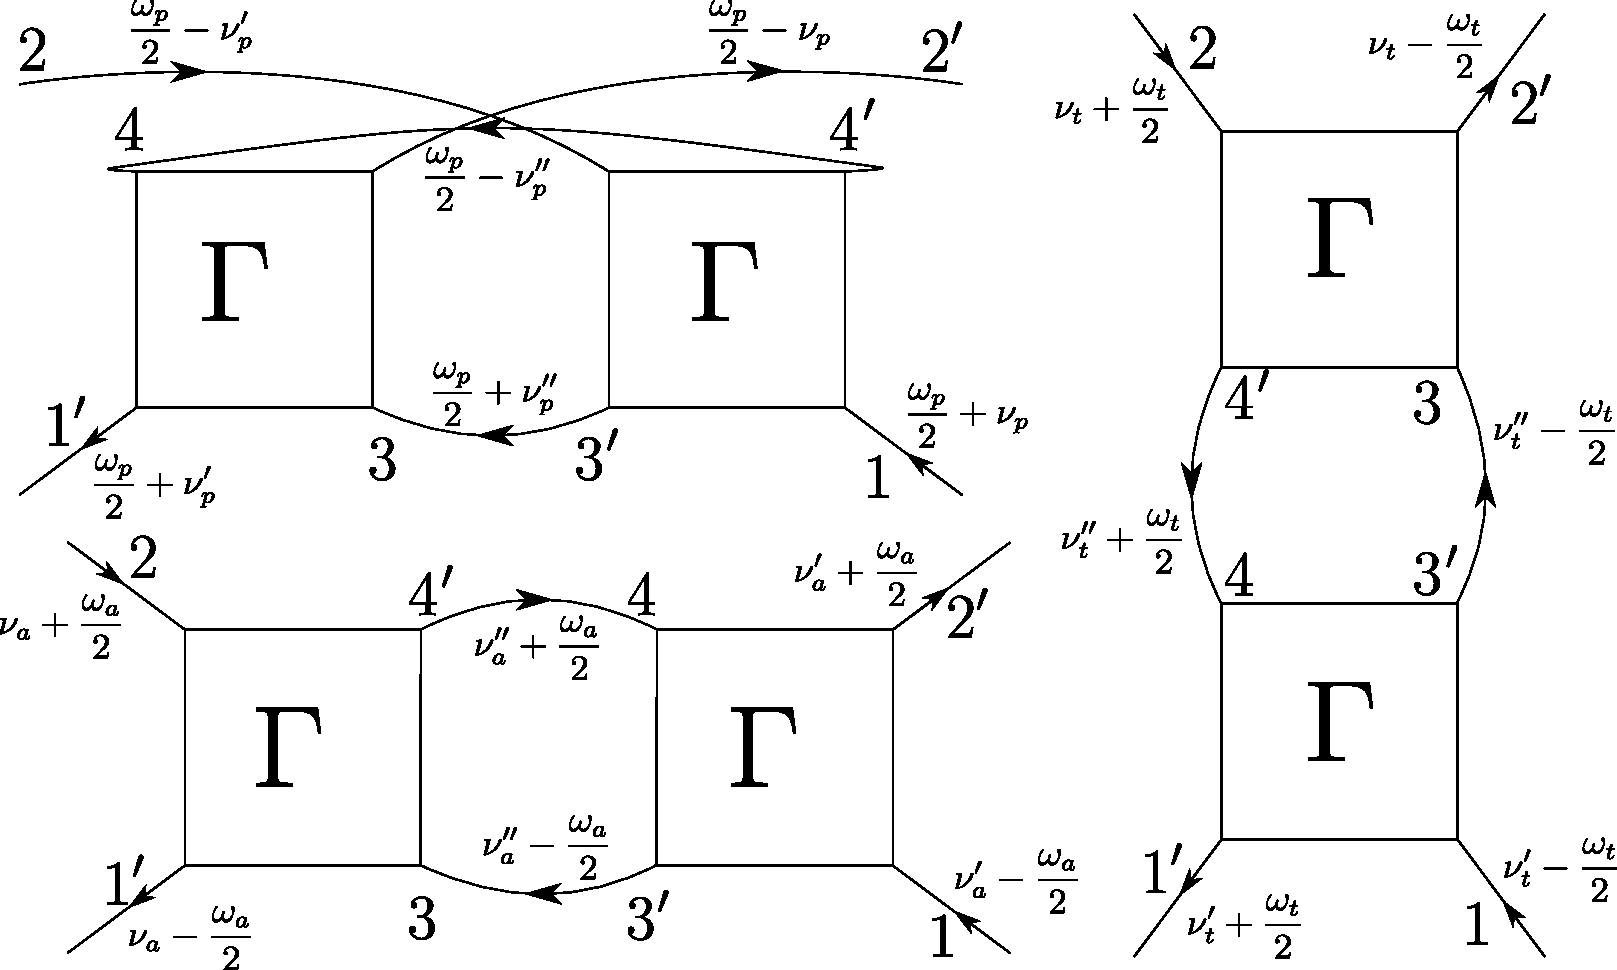
\includegraphics[width=\textwidth]{all-Bubbles.pdf}
	\caption{Bubbles in the respective channels}
\end{figure}




Thus, first of all, we have the frequency arguments that go into both propagators of  the bubble.  Now, as for the sole bubbles, their Keldysh structure gets simplified thanks to the causality constraint imposed by $G^{1|1}=0$. Thus, from the possible total of 16 Keldysh components, only 9 are not always zero and, if one chooses the following convention to define the indexation, these are the same for all channels, though the Keldysh structure of these elements not necessarily have to be the same. More precisely, the bubbles in the p-channel have a slightly different structure than the a- and t-channels that, due to their "conjugacy", take exactly the same structure.

For the a-channel, we have
\begin{align}
\Pi_a^{\alpha_3\alpha_4|\alpha'_3\alpha'_4} &= G^{\alpha_3|\alpha'_3}\left(\nu''_a-\frac{\omega_a}{2}\right)G^{\alpha_4|\alpha'_4}\left(\nu''_a+\frac{\omega_a}{2}\right)\\
\begin{pmatrix}
0  & 1  & 2   & 3\\
4  & 5  & 6   & 7\\
8  & 9  & 10 & 11\\
12& 13&14 & 15
\end{pmatrix} &=
\begin{pmatrix}
11|11 & 11|12 & 11|21 & 11|22 \\
12|11 & 12|12 & 12|21 & 12|22\\
21|11 & 21|12 & 21|21 & 21|22\\
22|11 & 22|12 & 22|21 & 22|22
\end{pmatrix} = \begin{pmatrix}
0    & 0    & 0    & AA \\
0    & 0    & AR & AK\\
0    & RA & 0    & KA\\
RR & RK & KR & KK
\end{pmatrix},
\label{eq:Pia}
\end{align}

for the p-channel
\begin{align}
\Pi_p^{\alpha_3\alpha_4|\alpha'_3\alpha'_4} &= G^{\alpha_3|\alpha'_3}\left(\frac{\omega_p}{2}+\nu''_p\right)G^{\alpha_4|\alpha'_4}\left(\frac{\omega_p}{2}-\nu''_p\right)\\
\begin{pmatrix}
0  & 1  & 2   & 3\\
4  & 5  & 6   & 7\\
8  & 9  & 10 & 11\\
12& 13&14 & 15
\end{pmatrix} &=
\begin{pmatrix}
11|11 & 11|12 & 11|21 & 11|22 \\
12|11 & 12|12 & 12|21 & 12|22\\
21|11 & 21|12 & 21|21 & 21|22\\
22|11 & 22|12 & 22|21 & 22|22
\end{pmatrix} = \begin{pmatrix}
0    & 0    & 0    & AA \\
0    & 0    & AR & AK\\
0    & RA & 0    & KA\\
RR & RK & KR & KK
\end{pmatrix},
\label{eq:Pip}
\end{align}

and, lastly, for the t-channel, the same as for the a-channel:
\begin{align}
\Pi_t^{\alpha_3\alpha_4|\alpha'_3\alpha'_4} &= G^{\alpha_3|\alpha'_3}\left(\nu''_t-\frac{\omega_t}{2}\right)G^{\alpha_4|\alpha'_4}\left(\nu''_t+\frac{\omega_t}{2}\right)\\
\begin{pmatrix}
0  & 1  & 2   & 3\\
4  & 5  & 6   & 7\\
8  & 9  & 10 & 11\\
12& 13&14 & 15
\end{pmatrix} &=
\begin{pmatrix}
11|11 & 11|12 & 11|21 & 11|22 \\
12|11 & 12|12 & 12|21 & 12|22\\
21|11 & 21|12 & 21|21 & 21|22\\
22|11 & 22|12 & 22|21 & 22|22
\end{pmatrix} = \begin{pmatrix}
0    & 0    & 0    & AA \\
0    & 0    & AR & AK\\
0    & RA & 0    & KA\\
RR & RK & KR & KK
\end{pmatrix}.
\label{eq:Pit}
\end{align}

In the case of $\dot{\Pi}_r$, one needs to of course replace $GG \rightarrow GS+SG$.

Note that, choosing this structural convention for the bubbles, one attains internal Keldysh structures that are exactly equal, independent of the channel. However, the way the legs are connected and, consequently, the functions that will be defined below do differ among the three channels. These functions are a devise to exploit the zeroes in the bubbles \textit{and}, simultaneously, the fact that one only needs to store $n_{K_i}$ Keldysh components per diagrammatic class.
These aforementioned functions are a devise to exploit the zeros in the bubbles \textit{and}, simultaneously, the fact that one only needs to store $n_{K_i}$ Keldysh components per diagrammatic class. These are functions that then, based on the Keldysh index, $i_0$, of the left hand side of Eq.~\eqref{eq:derivativeOfgamma} (i.e. $i_0\in\{0,\dots, n_{K_i}\}$ and the Keldysh index, $i_2$, of the list of non zero entries of the bubbles (i.e. $i_2\in\{3, 6, 7, 9, 11, 12, 13, 14, 15\}$)  determine precisely the corresponding components $i_1$ and $i_3$ for the vertices left and right of the bubble in Eq.~\eqref{eq:derivativeOfgamma}. Condensed into an equation, the statement is as follows:

\begin{equation}
\dot{\gamma_r}^{i_0}(\omega_r, \nu_r, \nu'_r) = \sum_{i_2\in BK} \int d\nu''_r \Gamma^{i^r_1(i_0, i_2)}(\omega_r, \nu_r, \nu''_r)  \dot{\Pi}_r^{i_2}(\nu_1^r, \nu_2^r)  \Gamma^{i^r_3(i_0, i_2)}(\omega_r, \nu''_r, \nu'_r),
\label{eq:fullgammaDerivative}
\end{equation}
where we have emphasized that the frequencies $\nu^r_{1}$ and $\nu^r_2$ that go into the bubbles depend on the channel, as depicted above in \Crefrange{eq:Pia}{eq:Pit}), that the indices $i_1$ and $i_3$ are functions of the other two indices and the way these are determined are also channel-dependent and $BK = \{3, 6, 7, 9, 11, 12, 13, 14, 15\}$.
Writing down the exact form of these functions is a straight-forward task, which requires the conversion of $i_0$ and $i_2$ into indices in the $\{1111, \dots, 2222\}$ set. To visualize the process, just look at the figures drawn above. There, it becomes apparent, that, for $i_0 \rightarrow \alpha'_1\alpha'_2|\alpha_1\alpha_2$ and $i_2 \rightarrow \alpha_3\alpha_4|\alpha'_3\alpha'_4$, the functions are as follows:

\begin{align}
i_1^a (\alpha'_1\alpha'_2|\alpha_1\alpha_2, \alpha_3\alpha_4|\alpha'_3\alpha'_4) &= \alpha'_1\alpha'_4| \alpha_3\alpha_2 \\
i_3^a (\alpha'_1\alpha'_2|\alpha_1\alpha_2, \alpha_3\alpha_4|\alpha'_3\alpha'_4) &= \alpha'_3\alpha'_2| \alpha_1\alpha_4 \\
i_1^p (\alpha'_1\alpha'_2|\alpha_1\alpha_2, \alpha_3\alpha_4|\alpha'_3\alpha'_4) &= \alpha'_1\alpha'_2| \alpha_3\alpha_4 \\
i_3^p (\alpha'_1\alpha'_2|\alpha_1\alpha_2, \alpha_3\alpha_4|\alpha'_3\alpha'_4) &= \alpha'_3\alpha'_4| \alpha_1\alpha_2 \\
i_1^t (\alpha'_1\alpha'_2|\alpha_1\alpha_2, \alpha_3\alpha_4|\alpha'_3\alpha'_4) &= \alpha'_4\alpha'_2| \alpha_3\alpha_2 \\
i_3^t (\alpha'_1\alpha'_2|\alpha_1\alpha_2, \alpha_3\alpha_4|\alpha'_3\alpha'_4) &= \alpha'_1\alpha'_3| \alpha_1\alpha_4
\end{align}
\subsection*{Structure of the internal bubble - diagrammatic classes' contributions}
Now, at this stage, the natural question to ask is how the \textit{diagrammatic} decomposition of Eq.~\eqref{eq:fullgammaDerivative} looks like i.e., given that $\dot{\gamma_r} = \sum_i \dot{K_i^r}$, what are the diagrammatic classes that contribute to each of these derivatives? It should by now be clear that not all classes can contribute to all derivatives, since, for instance, diagrams in the $K_3$ class, by definition, do not fulfill the requirement of having, say, two lines connected to the same vertex on one side. Thus, no terms with $K_3$ can appear in $\dot{K_1}$.
The natural thing to do at this stage is, basically, classify by sides and lines connected to one vertex, what classes fulfill the requirements to contribute, at least on one side, to which ones.
Thus, one can establish the following categorization:

\begin{center}
\renewcommand{\tabcolsep}{5pt} 
\renewcommand{\arraystretch}{1.2}
\begin{tabular}{| c| | c | c|} 
\hline
          &  L & R \\ 
          \hline\hline
 SV   & $\Gamma_0$, $K_1^r$, $\bar{K_2^r}$ & $\Gamma_0$, $K_1^r$, $K_2^r$\\ 
  DV & $K_2^r$, $K_3^r$, $\gamma_{\bar{r}}$  & $\bar{K_2^r}$, $K_3^r$, $\gamma_{\bar{r}}$\\ 
 \hline
\end{tabular}
\end{center}
Here, SV and DV stand for ''same vertex'' and ''different vertices'', alluding to whether or not both lines to the right (R) of the left (L) of the vertex connect to the same or to different vertices. 
$\Gamma_0$ is the bare vertex.
The inclusion already of $\gamma_{\bar{r}}$ is due to the foreshadowing of the multi-loop iterative loop i.e., we will be interested in feeding back diagrams of channels $\bar{r}$ to calculate higher loop order contributions to channel $r$.
Through this, one then gets the following Contribution Table to $\dot{K_i^r}$:

\begin{center}
\renewcommand{\tabcolsep}{5pt} 
\renewcommand{\arraystretch}{1.2}
\begin{tabular}{| c| | c | c|} 
\hline
          &  L & R \\ 
          \hline\hline
 $\dot{K_1^r}$  & $\Gamma_0$, $K_1^r$, $\bar{K_2^r}$ & $\Gamma_0$, $K_1^r$, $K_2^r$\\ 
 $\dot{K_2^r}$ & $K_2^r$, $K_3^r$, $\gamma_{\bar{r}}$  & $\Gamma_0$, $K_1^r$, $K_2^r$\\
 $\dot{\bar{K_2^r}}$ & $\Gamma_0$, $K_1^r$, $\bar{K_2^r}$ & $\bar{K_2^r}$, $K_3^r$, $\gamma_{\bar{r}}$\\ 
 $\dot{K_3^r}$ &  $K_2^r$, $K_3^r$, $\gamma_{\bar{r}}$   & $\bar{K_2^r}$, $K_3^r$, $\gamma_{\bar{r}}$\\
 \hline
\end{tabular}
\end{center}

What this table summarizes is the possible terms that can appear on the RHS of Eq.~\eqref{eq:derivativeOfgamma}, if one decomposes it into the diagrammatic classes.




\bibliography{bibliography}
\bibliographystyle{ieeetr}







\end{document}
